\documentclass[compress]{beamer}
\usepackage{ifthen,verbatim}

\newcommand{\isnote}{}
\xdefinecolor{lightyellow}{rgb}{1.,1.,0.25}
\xdefinecolor{darkblue}{rgb}{0.1,0.1,0.7}

%% Uncomment this to get annotations
%% \def\notes{\addtocounter{page}{-1}
%%            \renewcommand{\isnote}{*}
%% 	   \beamertemplateshadingbackground{lightyellow}{white}
%%            \begin{frame}
%%            \frametitle{Notes for the previous page (page \insertpagenumber)}
%%            \itemize}
%% \def\endnotes{\enditemize
%% 	      \end{frame}
%%               \beamertemplateshadingbackground{white}{white}
%%               \renewcommand{\isnote}{}}

%% Uncomment this to not get annotations
\def\notes{\comment}
\def\endnotes{\endcomment}

\setbeamertemplate{navigation symbols}{}
\setbeamertemplate{headline}{\mbox{ } \hfill
\begin{minipage}{5.5 cm}
\vspace{-0.75 cm} \small
\end{minipage} \hfill
\begin{minipage}{4.5 cm}
\vspace{-0.75 cm} \small
\begin{flushright}
\ifthenelse{\equal{\insertpagenumber}{1}}{}{Jim Pivarski \hspace{0.2 cm} \insertpagenumber\isnote/\pageref{numpages}}
\end{flushright}
\end{minipage}\mbox{\hspace{0.2 cm}}\includegraphics[height=1 cm]{../cmslogo} \hspace{0.1 cm} \includegraphics[height=1 cm]{../tamulogo} \hspace{0.01 cm} \vspace{-1.05 cm}}

\newcommand{\s}[1]{{\mbox{\scriptsize #1}}}

\begin{document}
%% \begin{notes}
%% \item This is the annotated version of my talk.
%% \item If you want the version that I am presenting, download the one
%% labeled ``slides'' on Indico (or just ignore these yellow pages).
%% \item The annotated version is provided for extra detail and a written
%% record of comments that I intend to make orally.
%% \item Yellow notes refer to the content on the {\it previous} page.
%% \item All other slides are identical for the two versions.
%% \end{notes}

\small

\begin{frame}
\frametitle{Status}
\renewcommand{\arraystretch}{1.4}
\begin{tabular}{p{0.5\linewidth} p{0.2\linewidth} p{0.2\linewidth}}
What? & Who? & When? \\\hline
Reco and trigger efficiency: get a number from a common source (or
quickly tag-and-probe $Z\to\mu\mu$) & me (probably) & nothing yet \\

Signal shape: fit resonances and gun & me & done (new) \\

Background shape: construct physically-meaningful templates and fit them & me & done \\

The fit: include all systematics and make upper limit plots & Vadim & looks good; improvements in pipeline \\

Understanding low-mass excess & Aysen & ? \\

Paper: introduction/motivation & me & done (new) \\

Paper: everything but the fit/limits & me & half-done \\

Paper: the fit and limits & Alexei & ? \\
\end{tabular}
\end{frame}

\begin{frame}
\frametitle{Reminder}
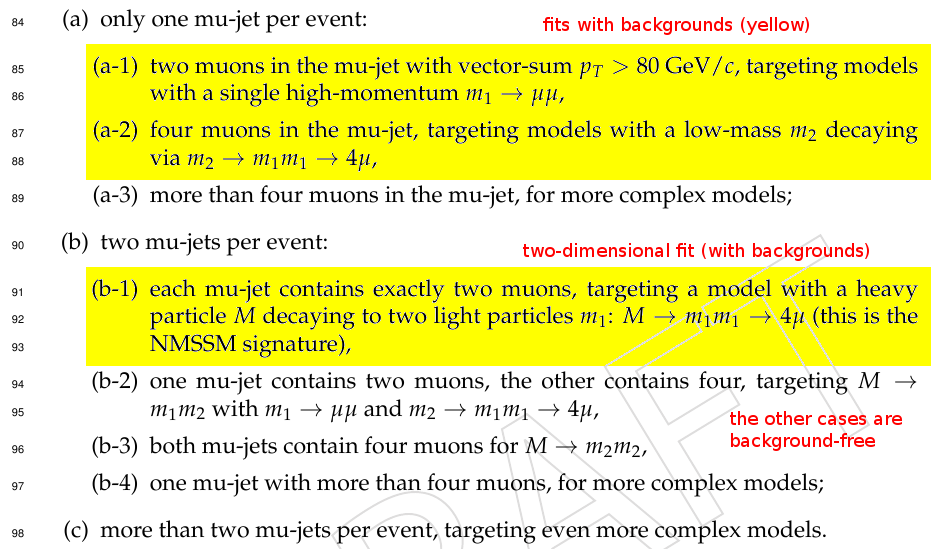
\includegraphics[width=\linewidth]{signal_regions.png}

\vspace{-0.4 cm}
\begin{tabular}{p{\linewidth}}
\\\hline
\end{tabular}

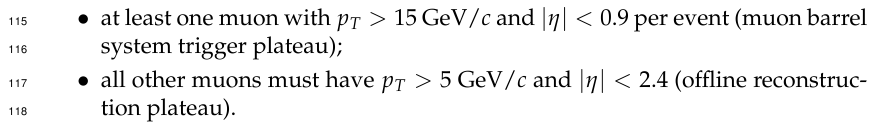
\includegraphics[width=\linewidth]{analysis_cuts.png}
\end{frame}

\begin{frame}
\frametitle{Signal shape}
\begin{itemize}
\item In writing this up, I noticed that the real shape in the endcap is double-Gaussian (quantified by $f_{0.07}$ below)
{\tiny
\begin{multline}
f(m) = p \bigg[ (1 - f_{0.07}) 
\left\{ \begin{array}{c l} \dfrac{1}{\sqrt{2\pi}\, \sigma} \exp\left(-(m - m_0)^2 / (2 \sigma^2)\right) & \mbox{if $(m - m_0)/\sigma > -\alpha$} \\
\dfrac{2}{5 \sigma} \exp\left(-\alpha^2/2\right)/(1 - \alpha^2 - (m-m_0)/\sigma) & \mbox{otherwise} \end{array} \right. \\
+ f_{0.07} \frac{1}{\sqrt{2\pi}\, 0.07} \exp\left(-(m - m_0)^2 / (2 \cdot 0.07^2)\right)\bigg]\mbox{.}
\end{multline}}

\vspace{-0.5 cm}
\item Core Gaussian same in barrel and endcap, data and MC (left)

\item 0.07~GeV/$c^2$ wide second Gaussian is relevant only in endcap (right)

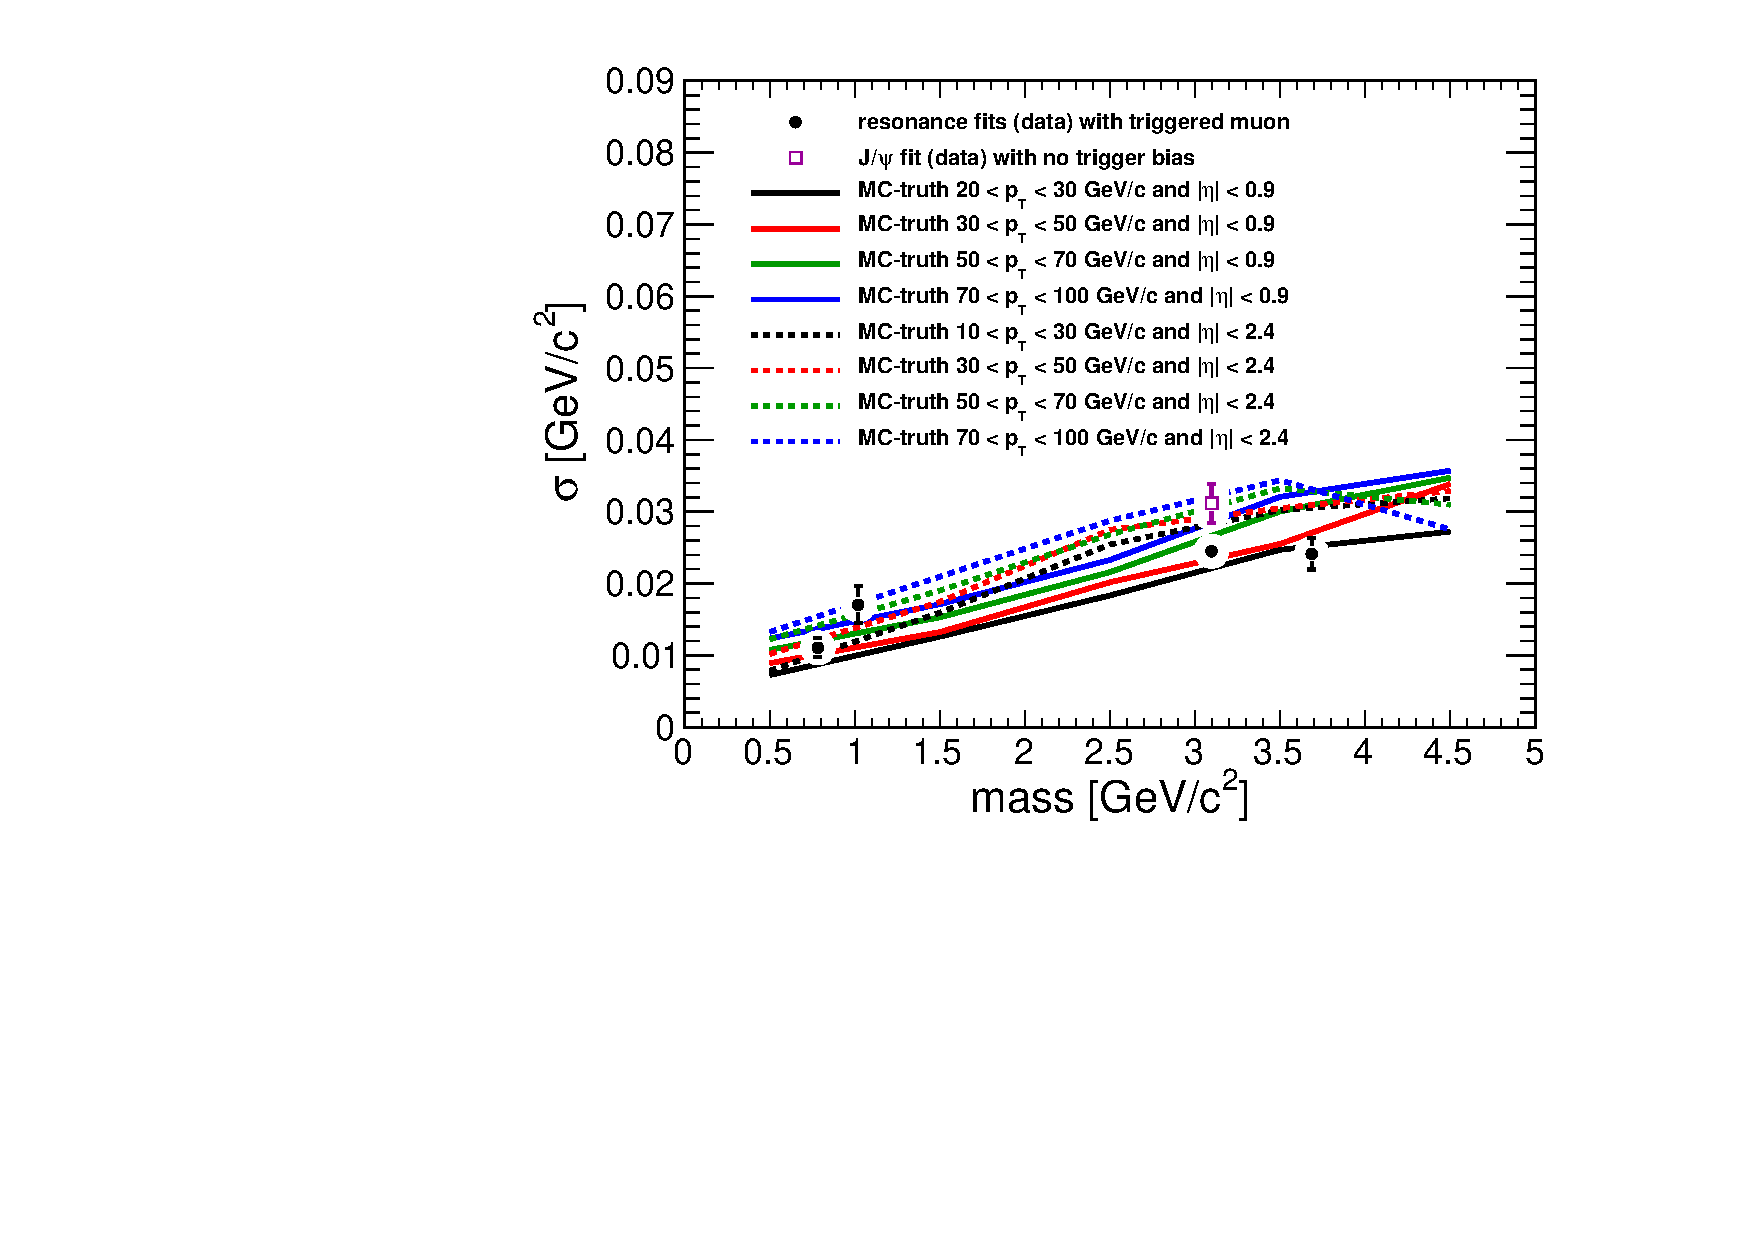
\includegraphics[width=0.5\linewidth]{resolution.pdf}
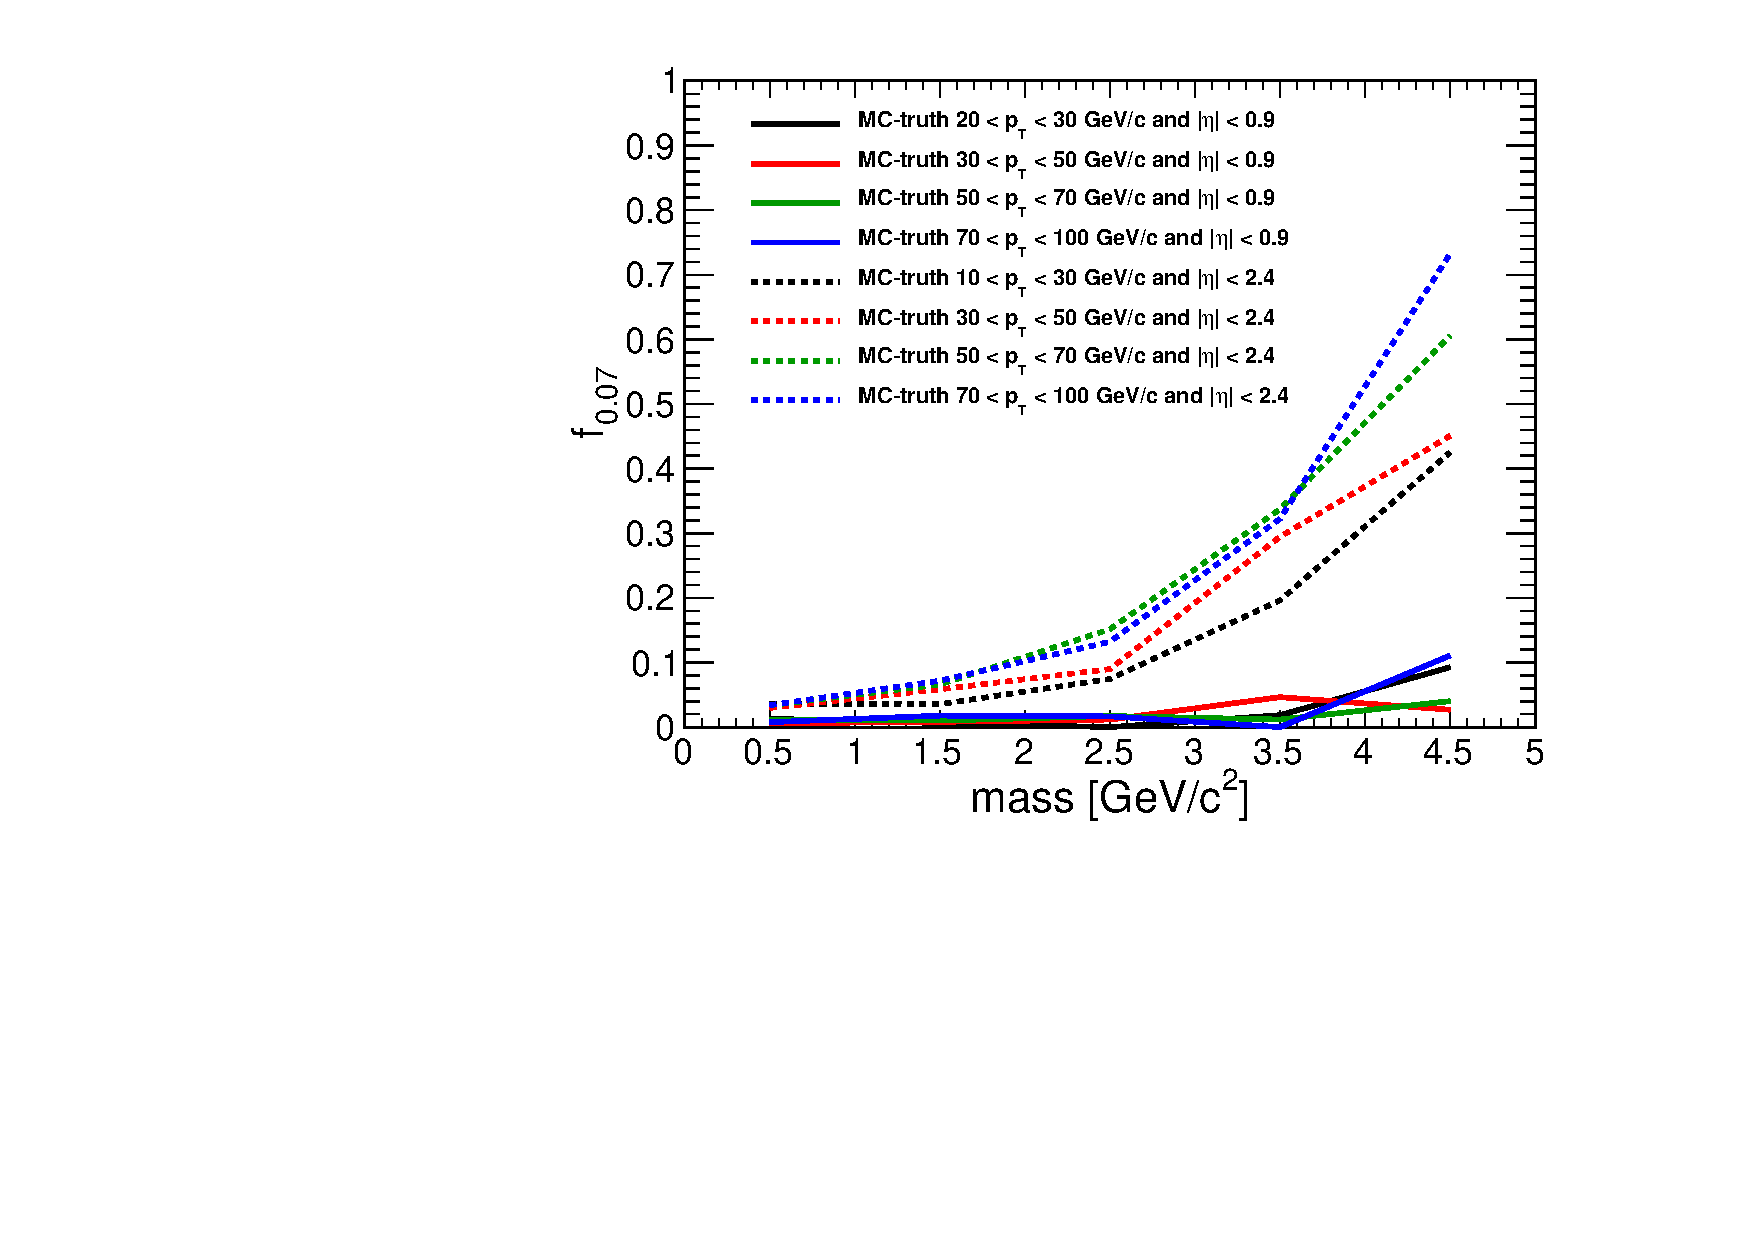
\includegraphics[width=0.5\linewidth]{resolution_f007.pdf}

\item Only information on Crystal Ball $\alpha = 2.04 \pm 0.11$ from data $J/\psi$ fit
\end{itemize}
\end{frame}

\begin{frame}
\frametitle{Signal shape}

Gallery of peaks in data (fit function on previous page with some
parameters fixed and an extra $p_0 + p_1 m$ linear background)

\vfill Most apply to the barrel only, since they must satisfy the
requirement of at least one $p_T > 15$~GeV/$c$, $|\eta| < 0.9$ muon

\vfill
\begin{columns}
\column{0.33\linewidth}
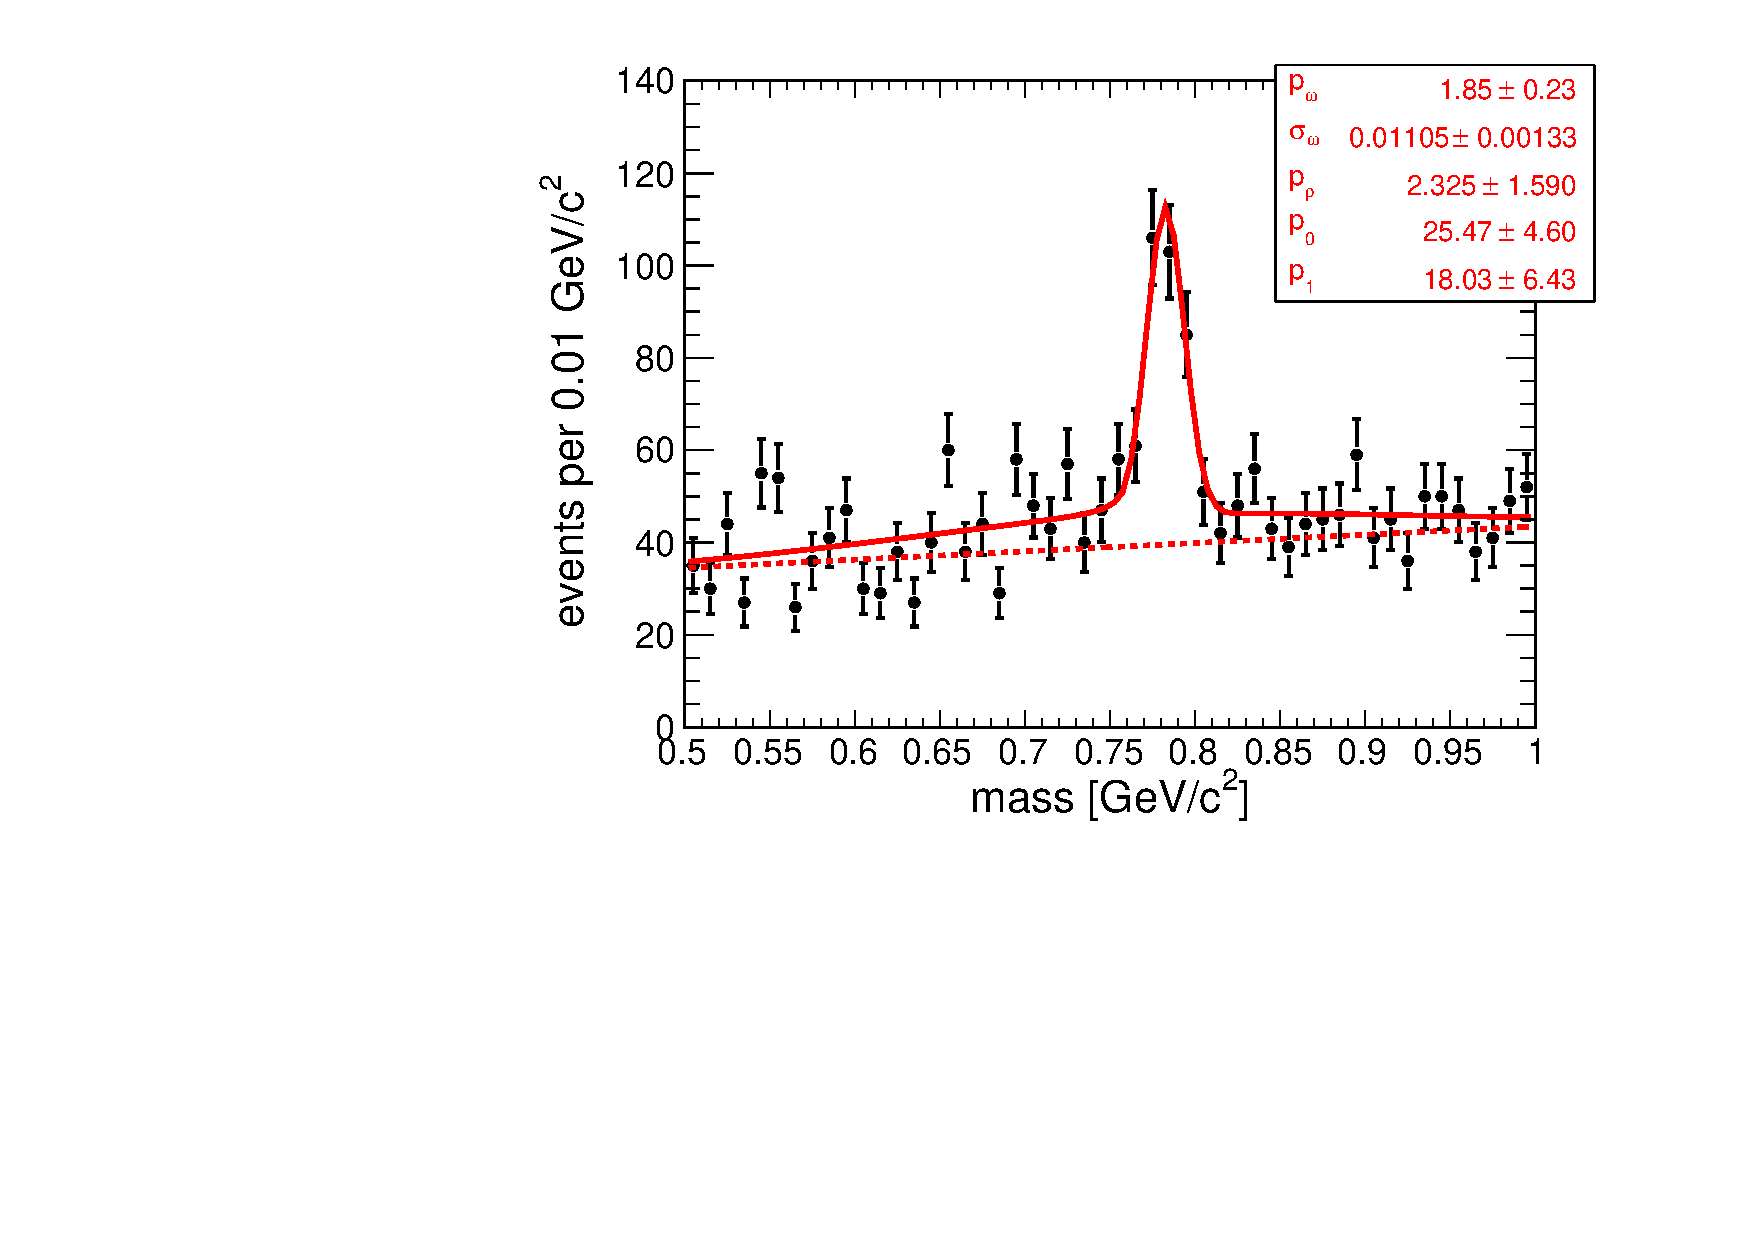
\includegraphics[width=\linewidth]{respeak_omega.pdf}

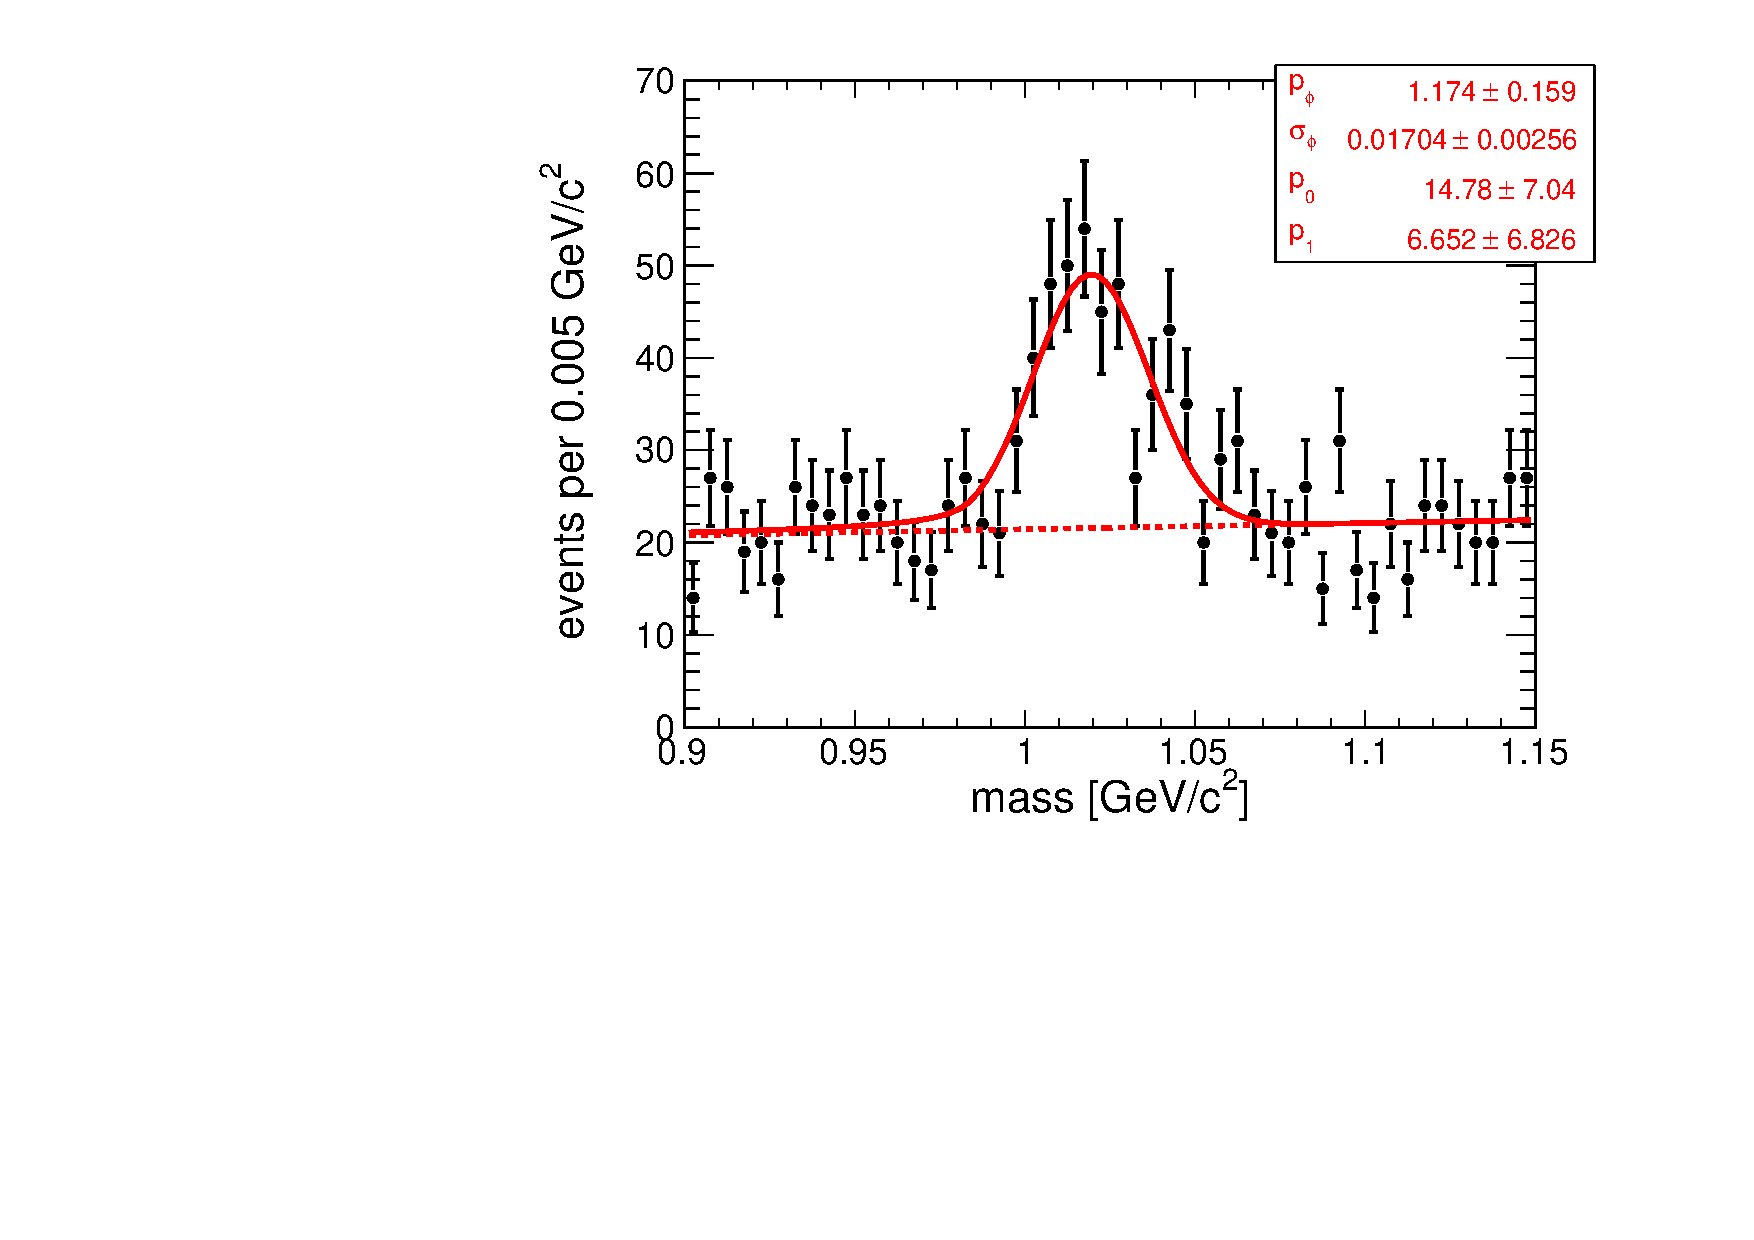
\includegraphics[width=\linewidth]{respeak_phi.pdf}

\column{0.33\linewidth}
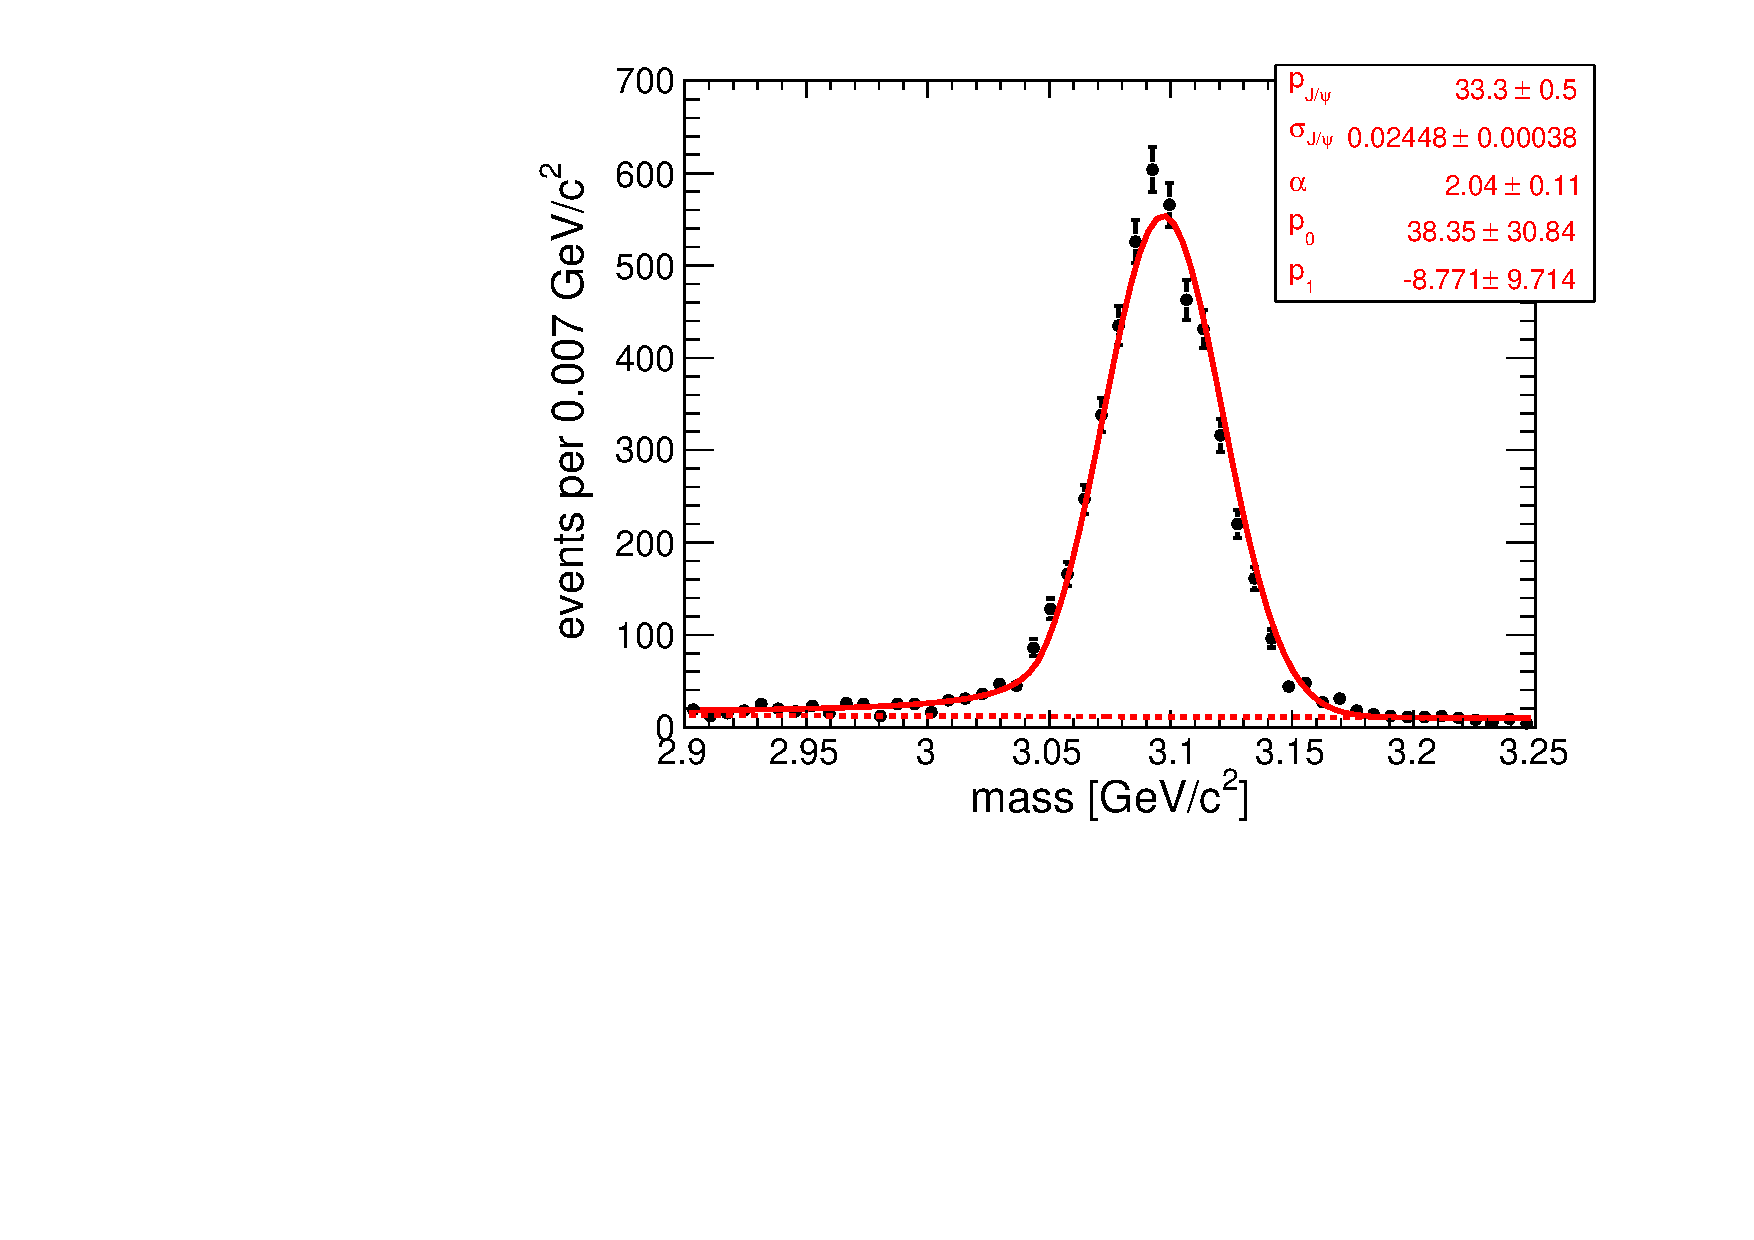
\includegraphics[width=\linewidth]{respeak_jpsi.pdf}

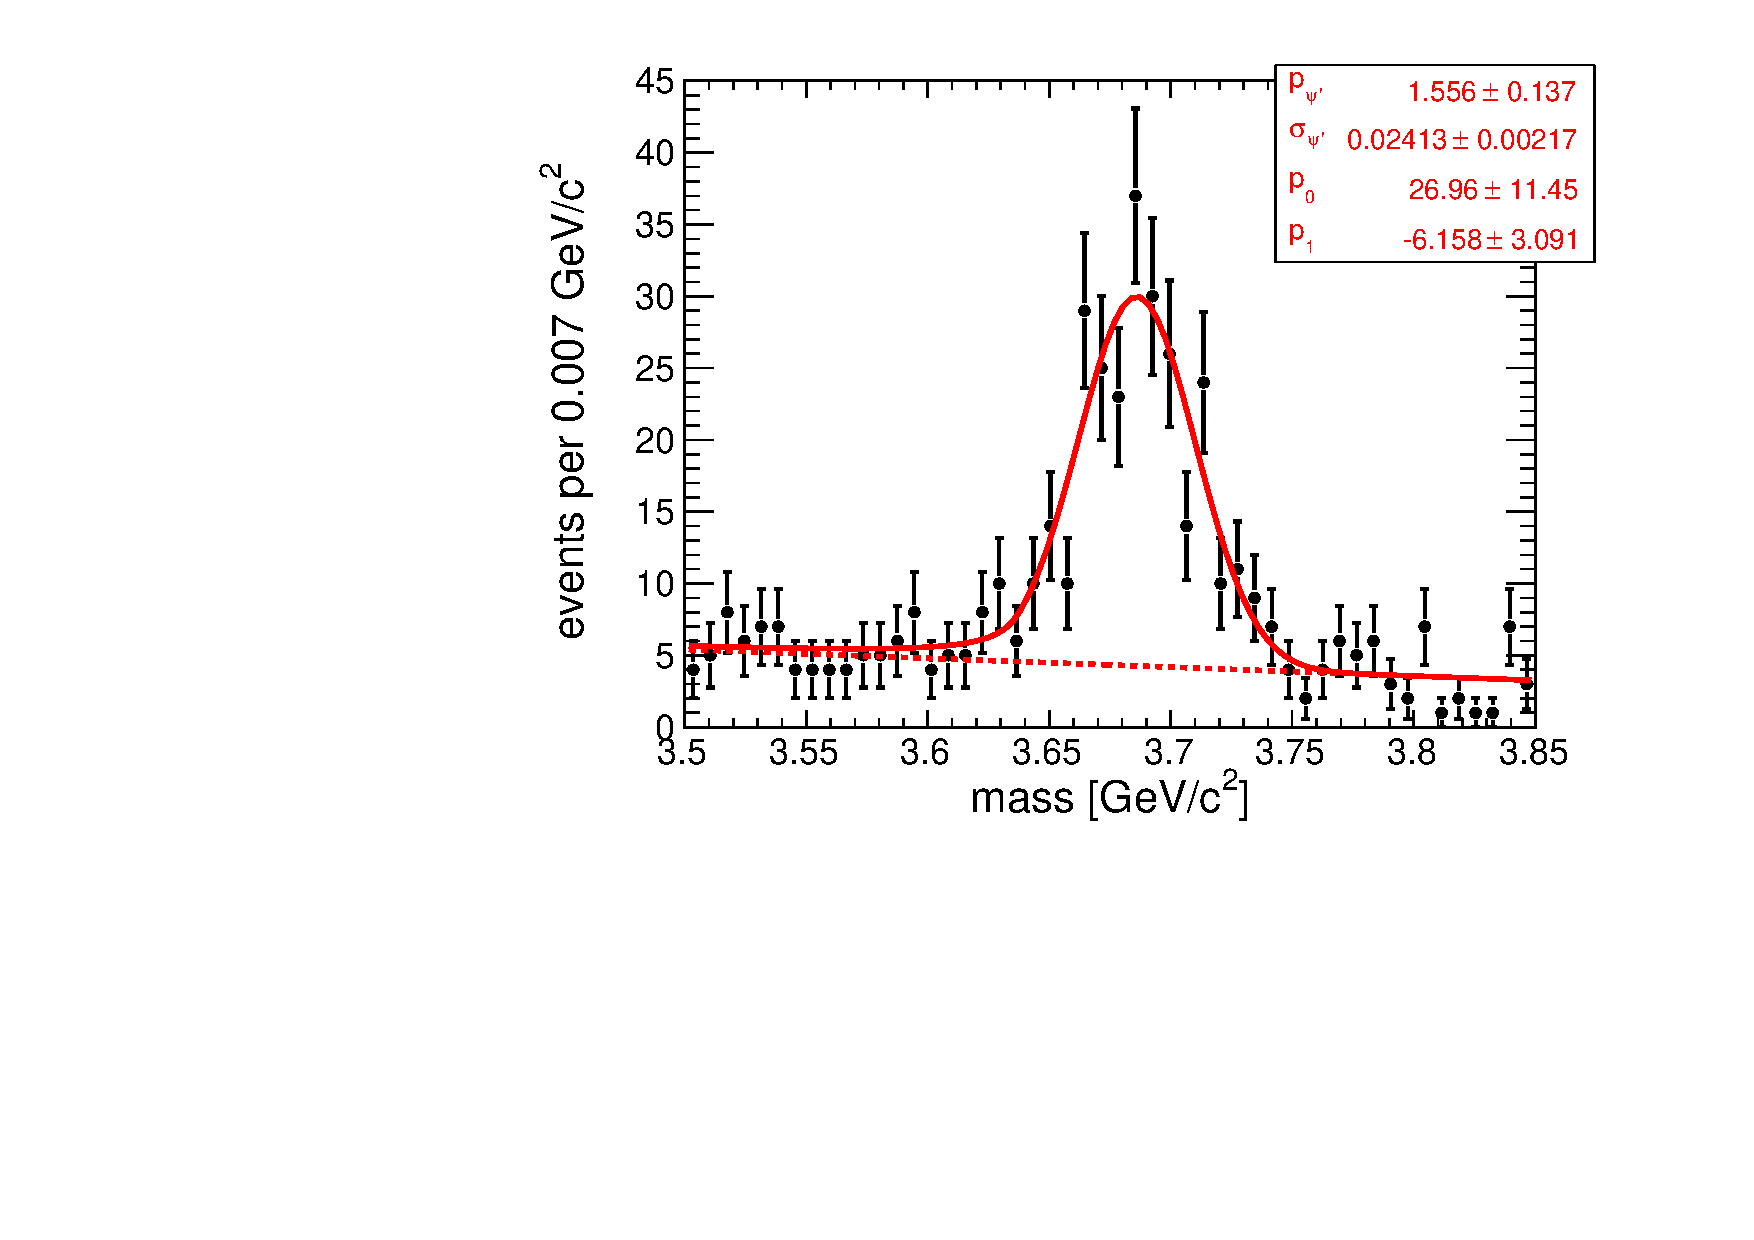
\includegraphics[width=\linewidth]{respeak_psiprime.pdf}

\column{0.33\linewidth}
This one (below) is the $J/\psi$ with a third muon to satisfy the trigger.  It
therefore applies to the whole $\eta$ range.

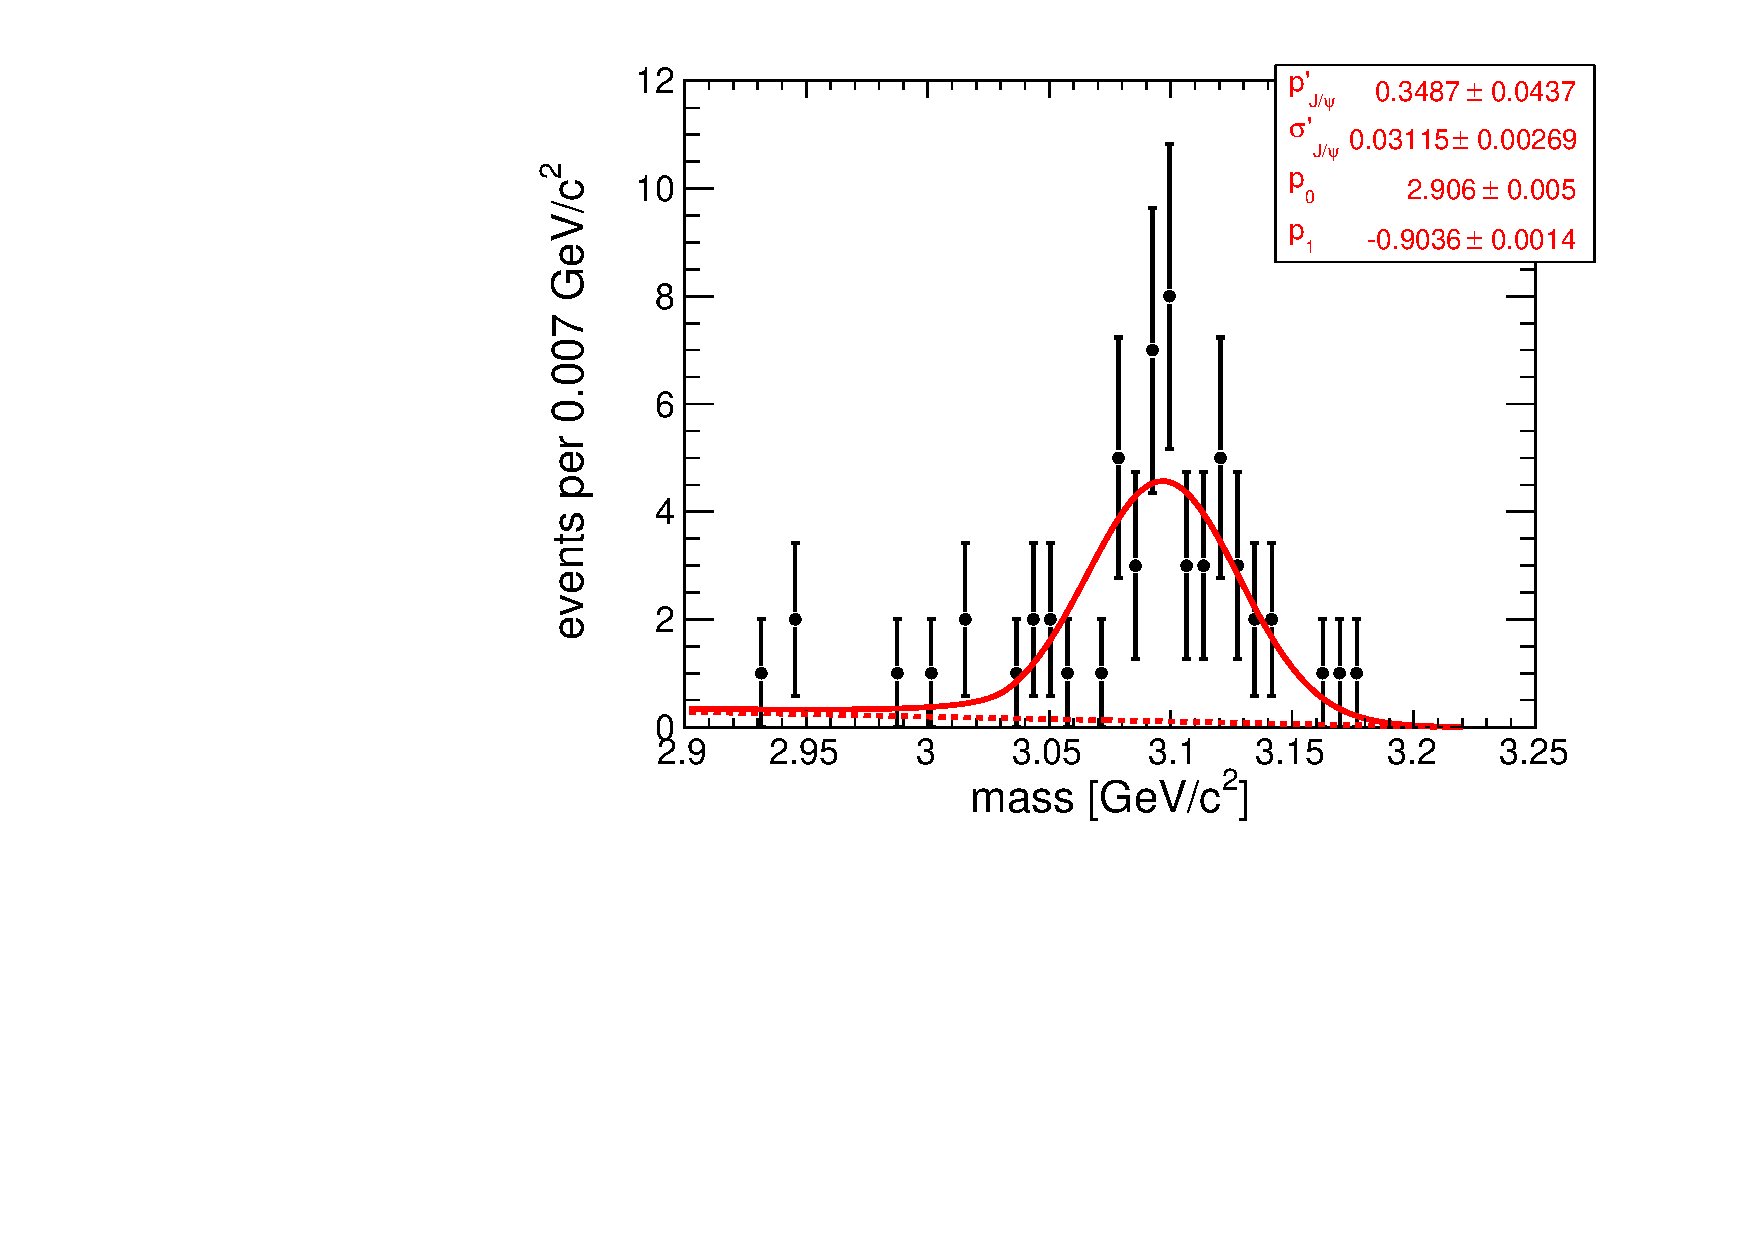
\includegraphics[width=\linewidth]{respeak_jpsi2.pdf}
\end{columns}
\end{frame}

\begin{frame}
\frametitle{For the fitter (signal part)}
\begin{itemize}
\item For all dimuon signal regions with $|\eta| < 0.9$ (a-1, a-2,
  triggered dimuon in b-1), the double-Gaussian term is unnecessary
  ($f_{0.07} = 0$)
\item For dimuons that are allowed in the whole range, we should either
\begin{itemize}
\item sample the $\eta$ distribution and set $f_{0.07}$ appropriately, or
\item simply let $f_{0.07}$ float in the signal-search.
\end{itemize}

\item We don't need to worry about the $p_T$ dependence

\item Extremes observed on the plots (page 3):

\begin{equation}
0.004 + 0.006 m < \sigma(m) < 0.011 + 0.007 m \mbox{ [GeV/$c^2$]}
\end{equation}

\begin{equation}
0 < f_{0.07}(m) < 0.04 + 0.008 m^3 \mbox{ [fraction of area]}
\end{equation}
\end{itemize}
\end{frame}

\begin{frame}
\frametitle{Dimuon studies}

{\tiny Drell-Yan output from Pythia output, rather than $Z$-scaling.
  All plots range 0.25--5~GeV/$c^2$ in 190 bins.  ``Low-mass'' is
  0.35--0.5~GeV/$c^2$, ``continuum'' is 1.1--2.9~GeV/$c^2$.
  $b\bar{b}$ cuts are: $Iso > 4.5\mbox{ GeV/$c$}\mbox{ \bf or }L_{xy}
  > 2\mbox{ mm}$.}


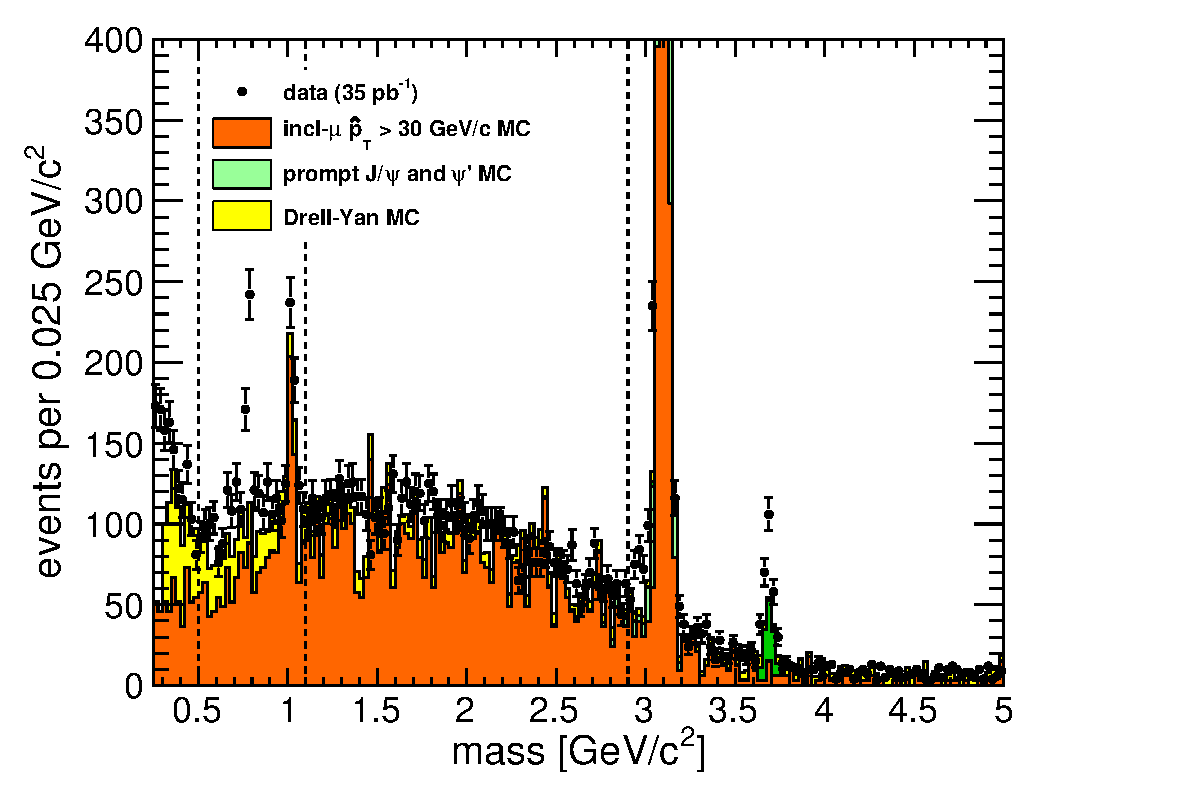
\includegraphics[width=0.33\linewidth]{support_mass_all.pdf}
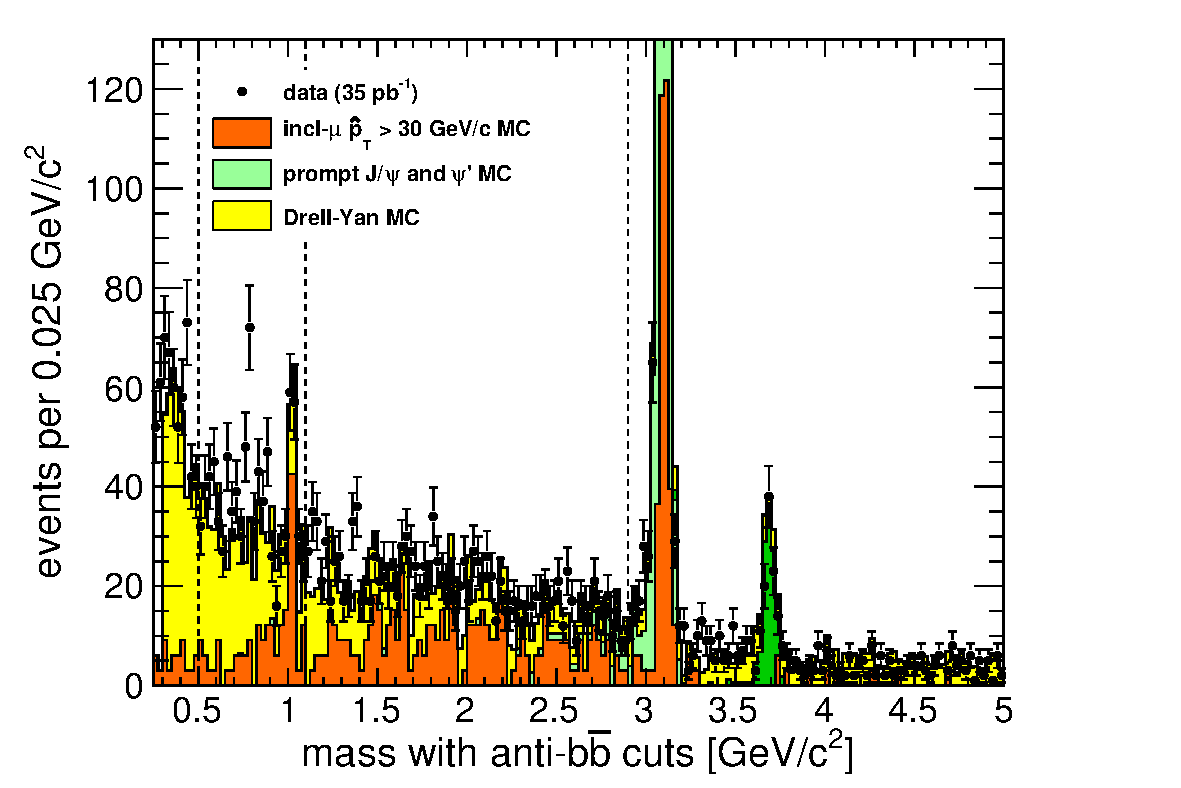
\includegraphics[width=0.33\linewidth]{support_mass_antibbbar.pdf}
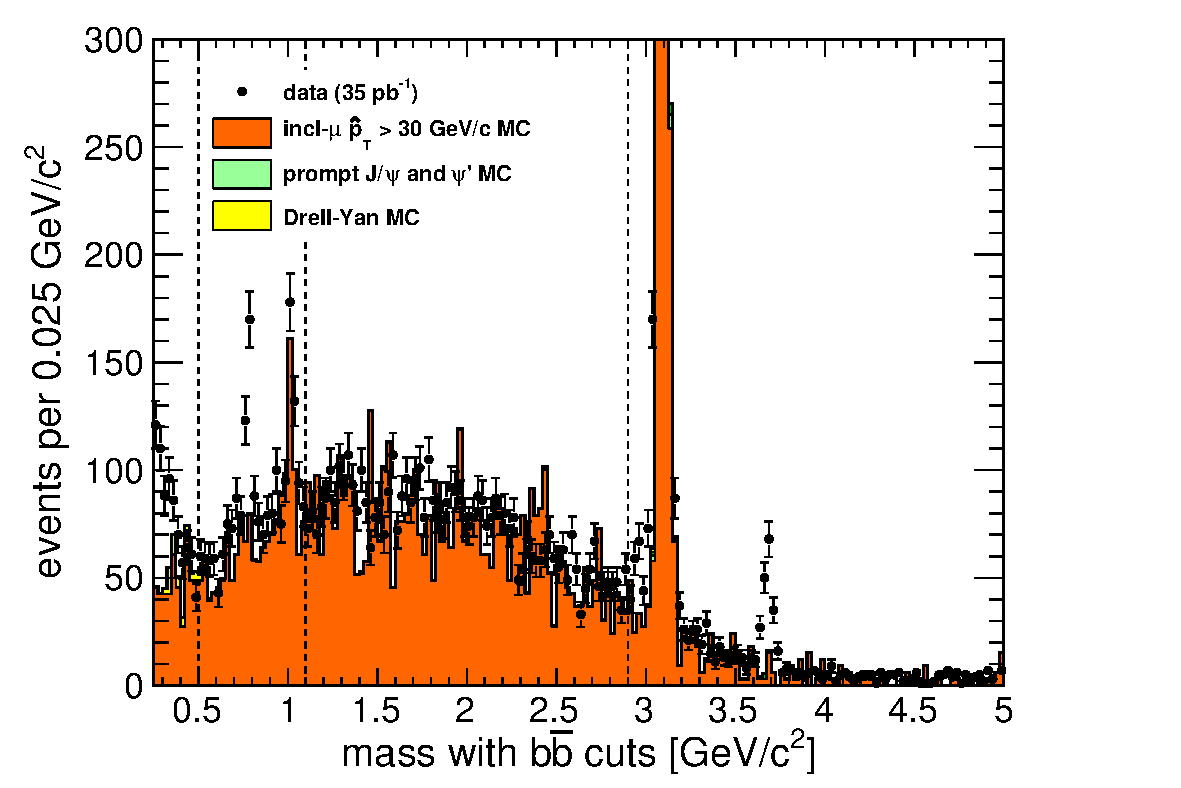
\includegraphics[width=0.33\linewidth]{support_mass_bbbar.pdf}

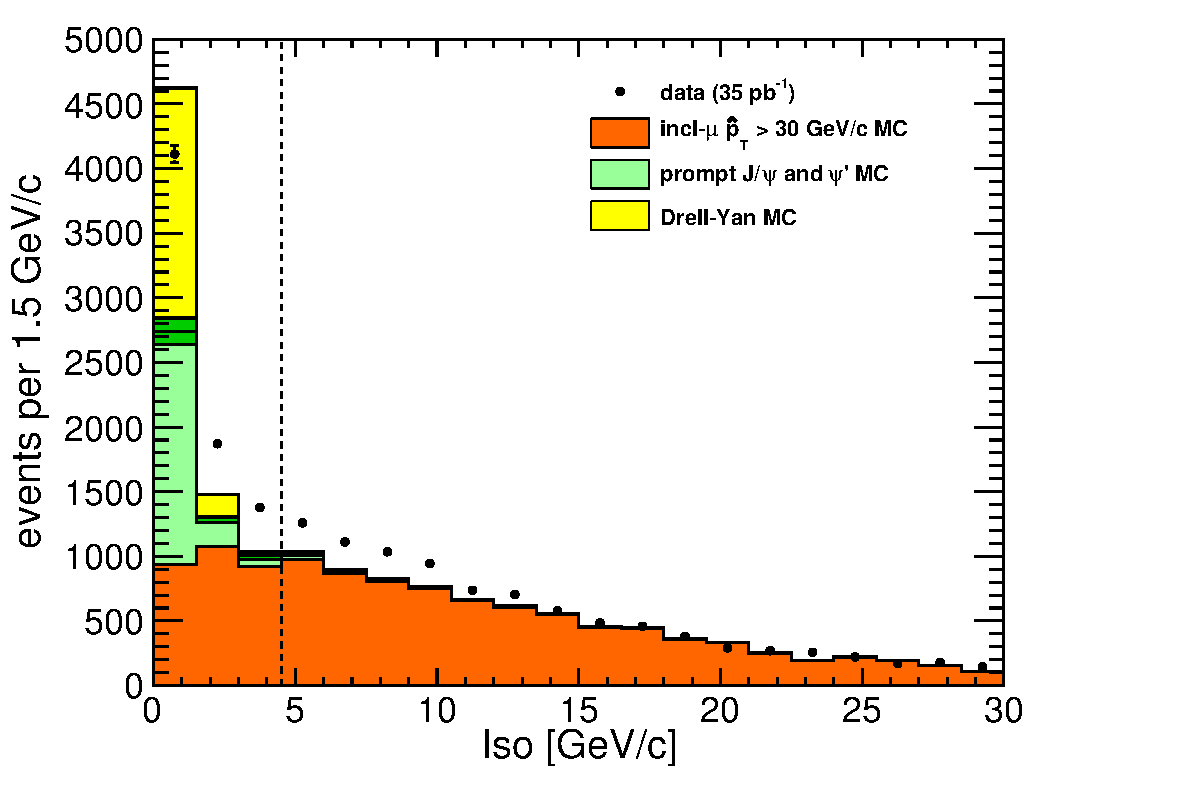
\includegraphics[width=0.33\linewidth]{support_iso_all.pdf}
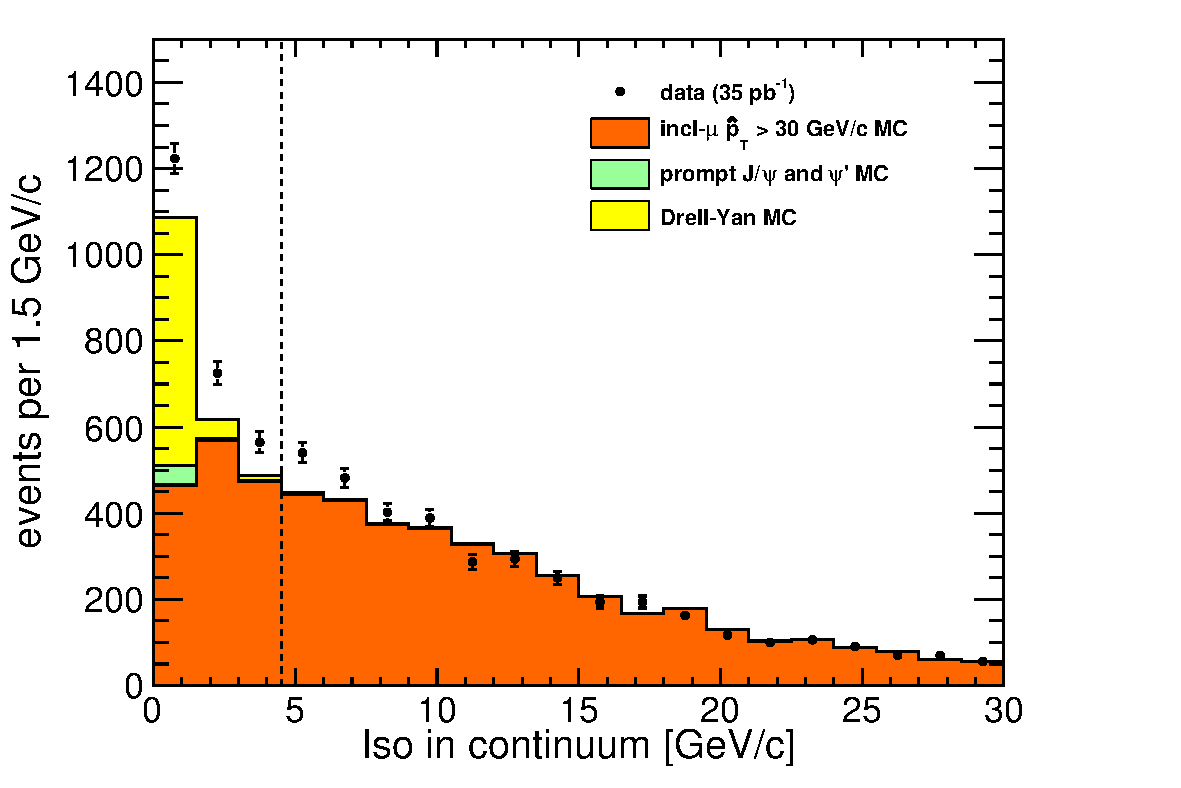
\includegraphics[width=0.33\linewidth]{support_iso_continuum.pdf}
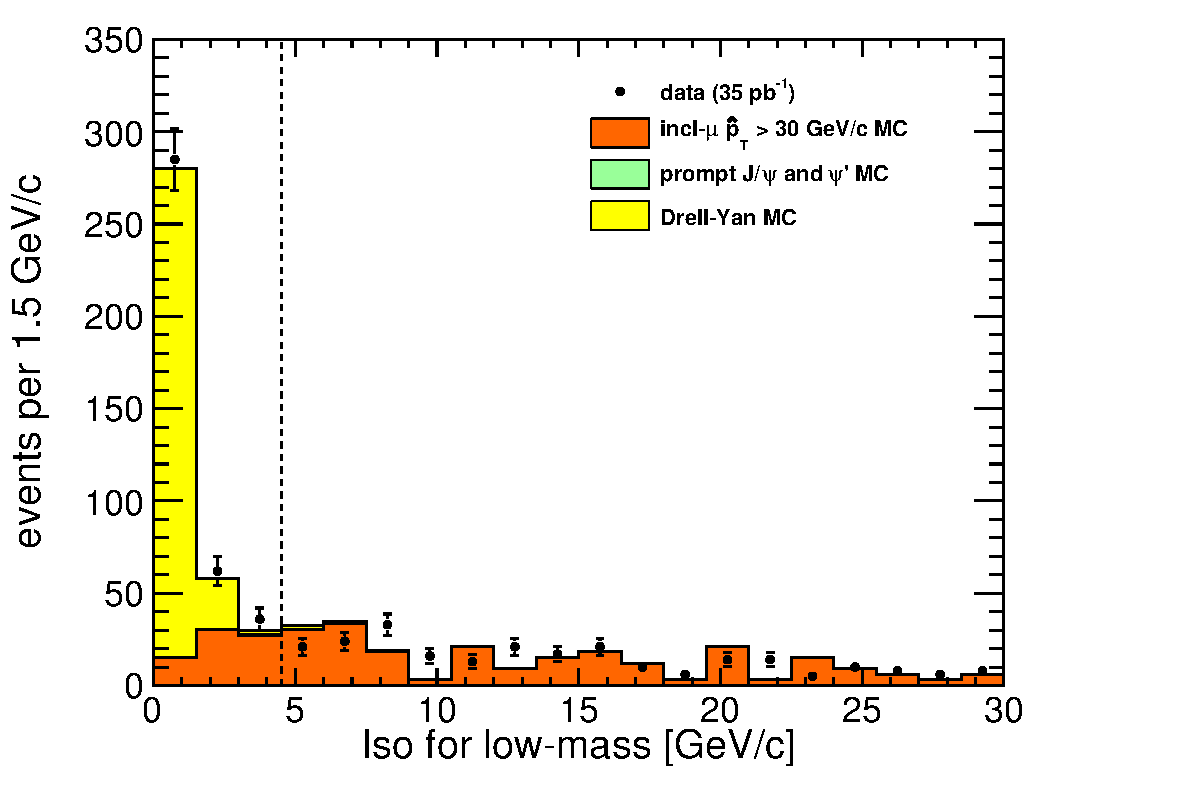
\includegraphics[width=0.33\linewidth]{support_iso_lowmass.pdf}

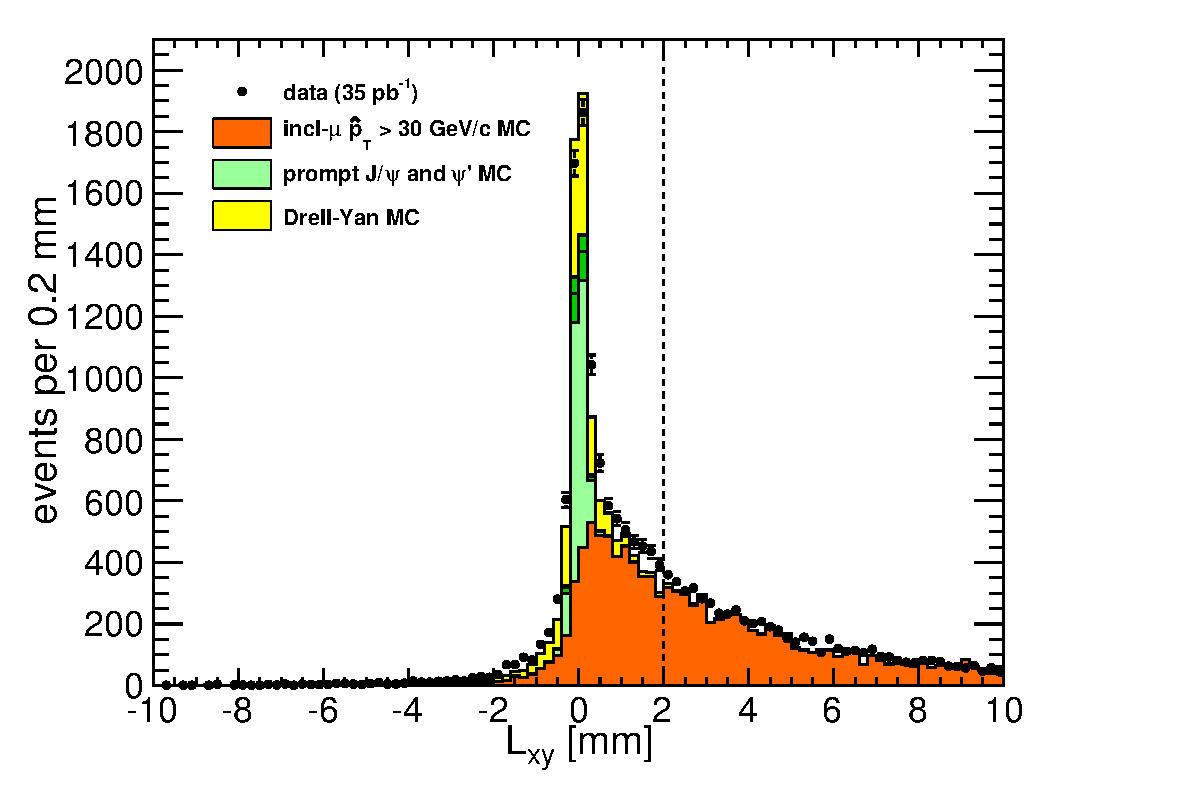
\includegraphics[width=0.33\linewidth]{support_lxy_all.pdf}
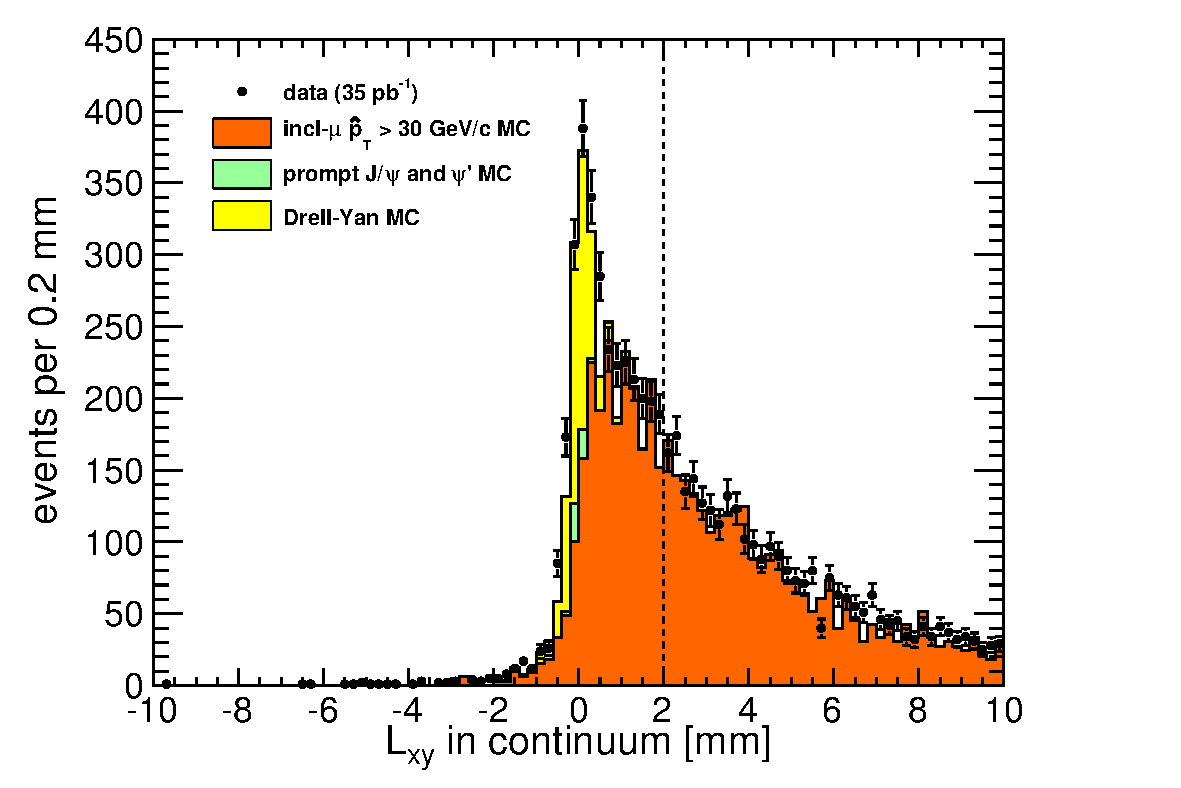
\includegraphics[width=0.33\linewidth]{support_lxy_continuum.pdf}
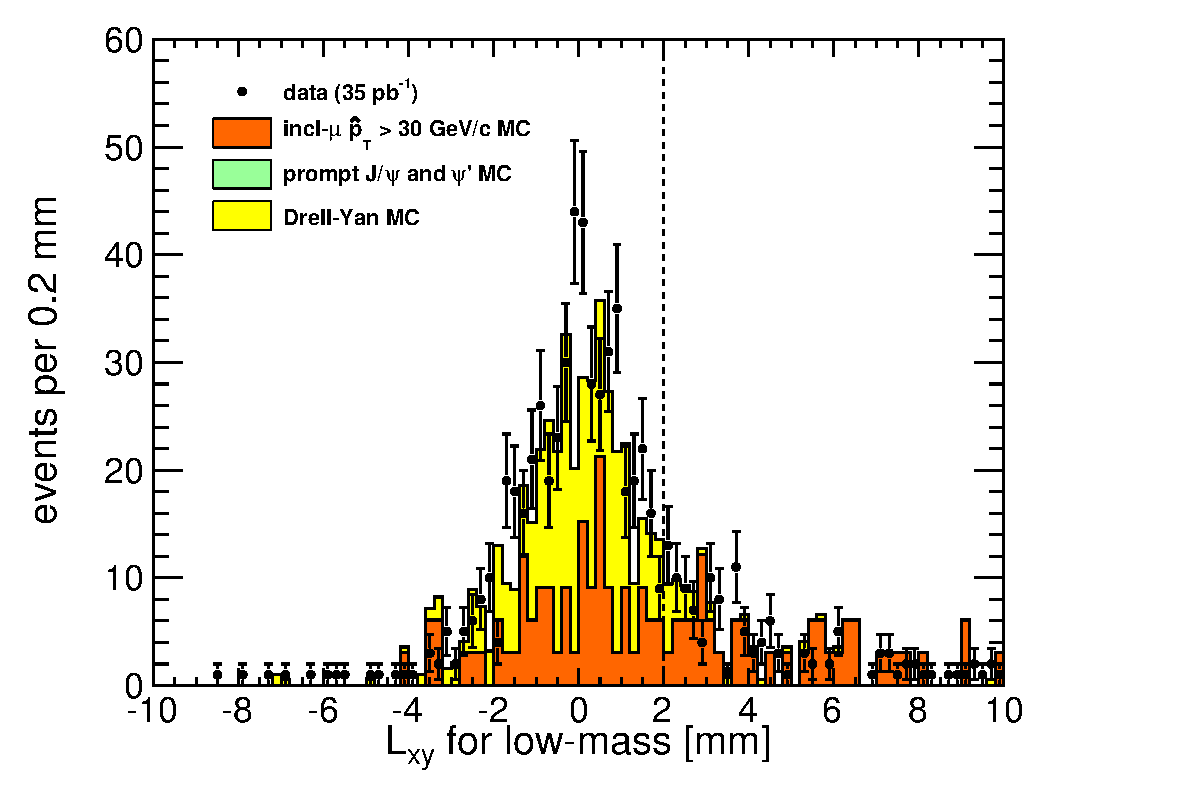
\includegraphics[width=0.33\linewidth]{support_lxy_lowmass.pdf}
\end{frame}

\begin{frame}
\frametitle{Dimuon studies}

\begin{itemize}
\item Understanding the low-mass region and the $b\bar{b}$ cuts will
  be important for defining mass templates, but not analyzing signal.

\item Scaling Drell-Yan by Pythia output fills in the anti-$b\bar{b}$
  cut region (why is Pythia calculation correct for low-mass but not
  for $Z$?)

\item Low-mass excess in $b\bar{b}$ is still not fully understood: is
  it possible to find photons in jets?  Perhaps identify the
  $b\bar{b}$ system by tagging the {\it other} $b$-quark, then ask for
  the $b$ with muons to be clean?

\item These $b\bar{b}$ cuts are uniformly efficient for MC $b\bar{b}$
  (left), and the $b\bar{b}$ and non-$b\bar{b}$ components scale
  proportionally with $p_T$ (right)
\end{itemize}

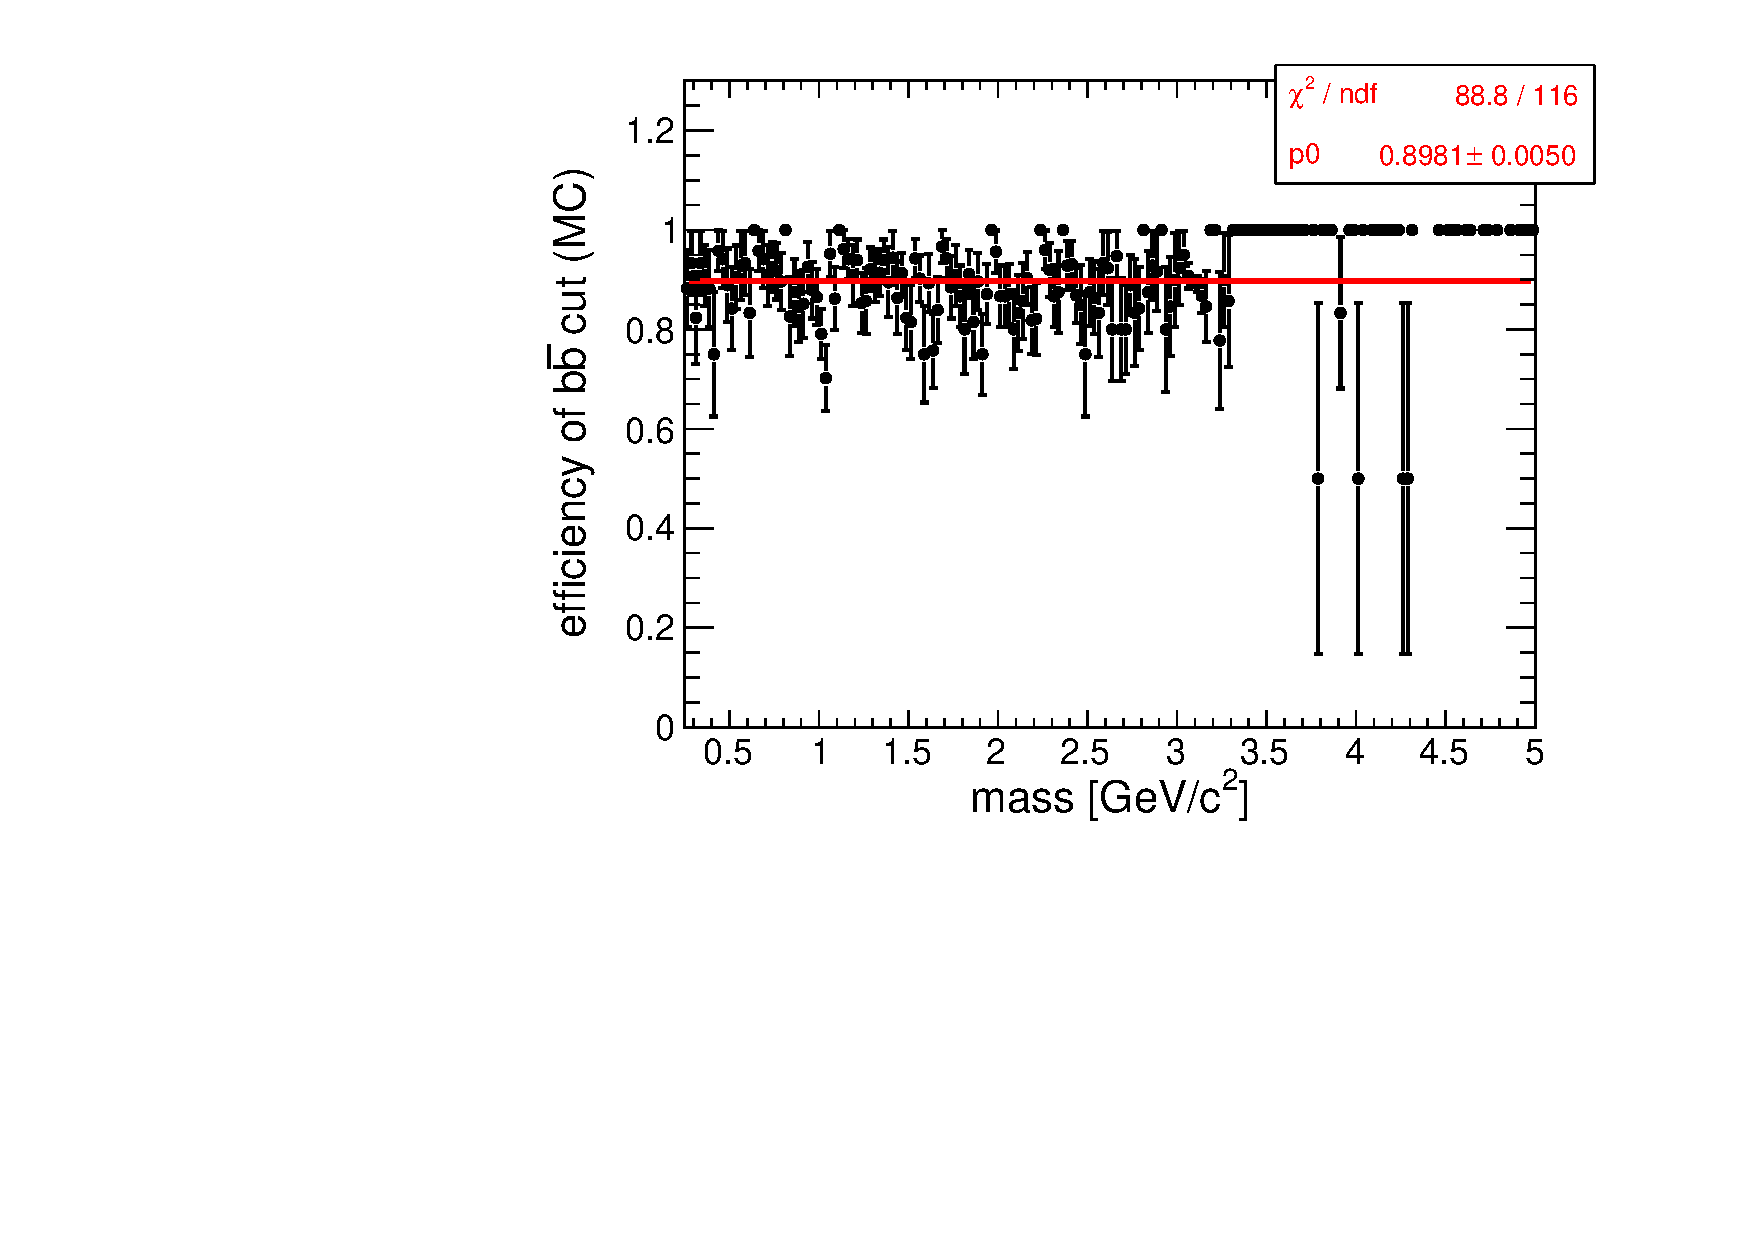
\includegraphics[width=0.5\linewidth]{support_bbbarcut_efficiency.pdf}
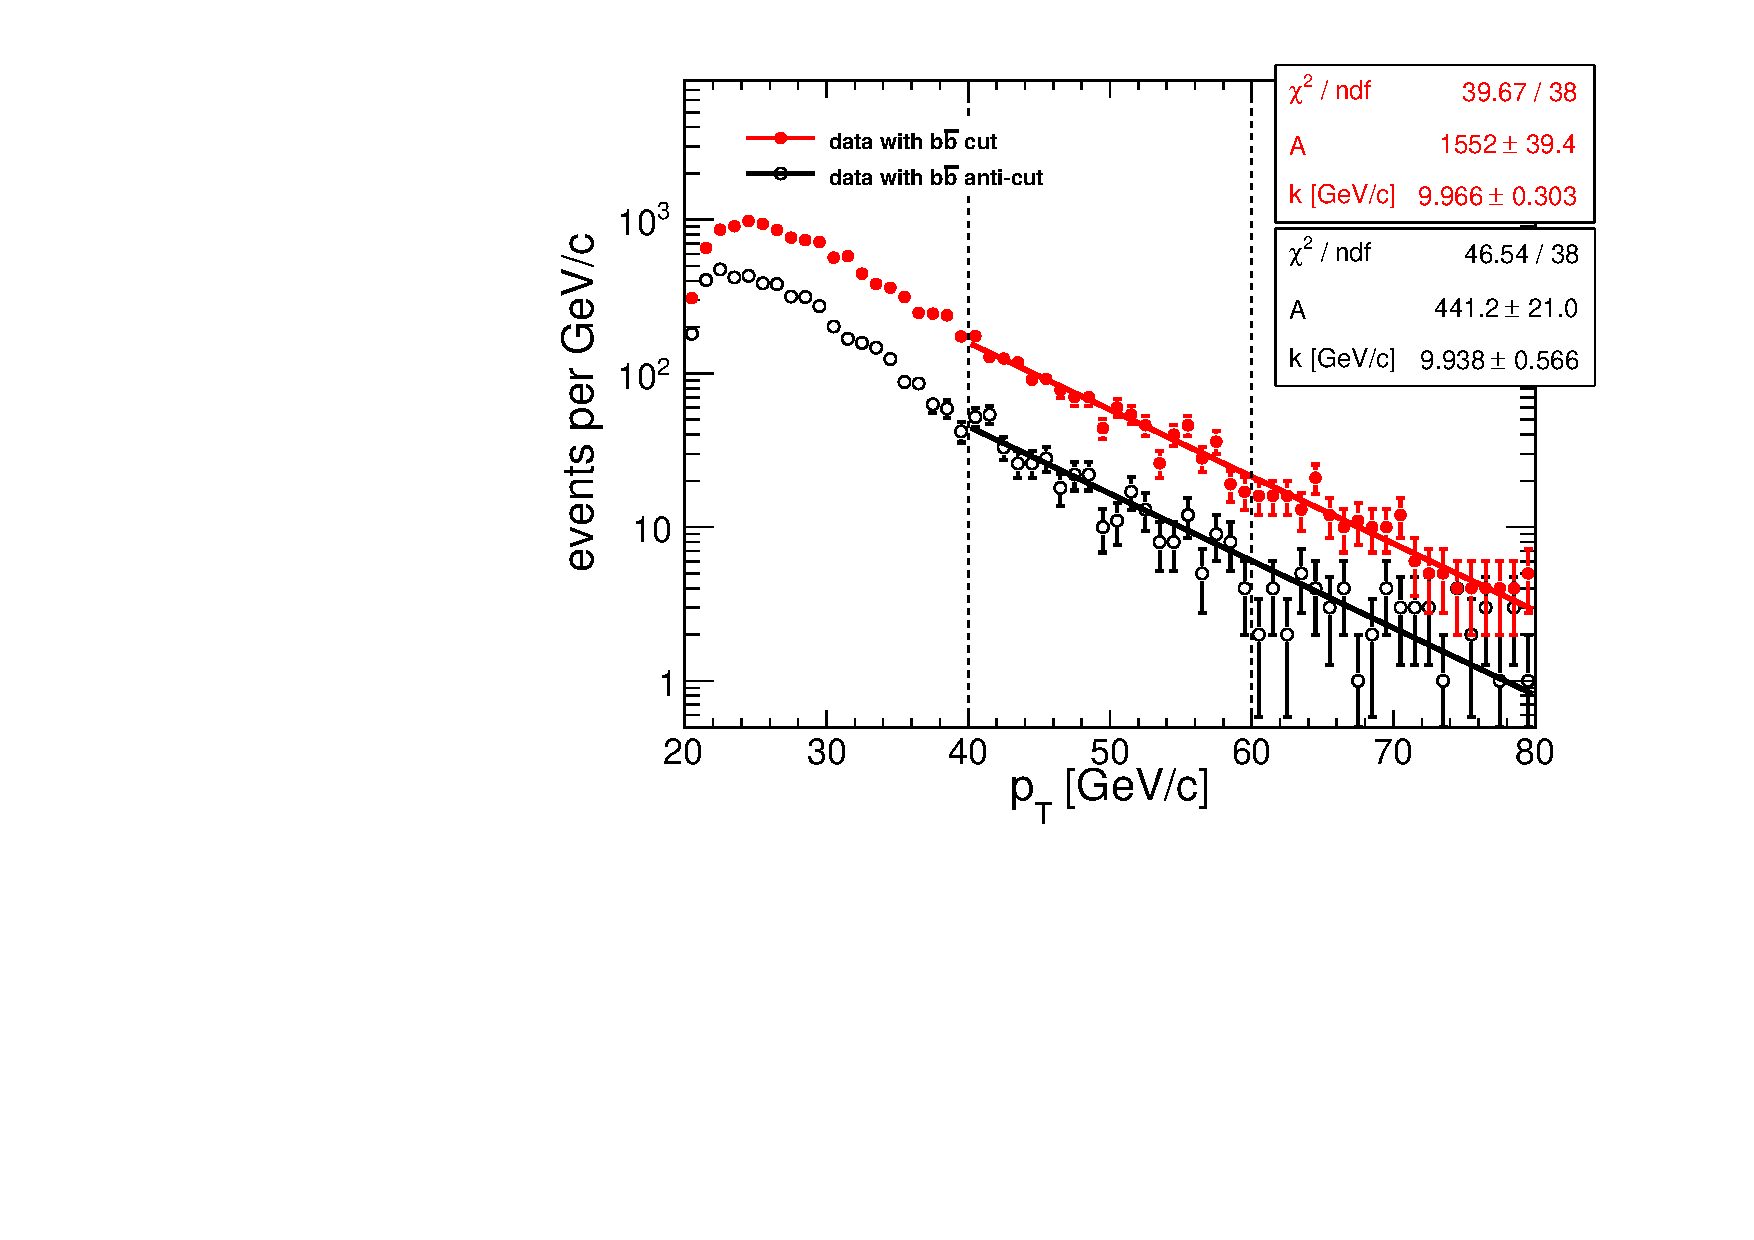
\includegraphics[width=0.5\linewidth]{support_bbbarcut_limits.pdf}
\end{frame}

\begin{frame}
\frametitle{Mass template for (a-1)}

\begin{itemize}
\item ``Background-enriched'' is $40 < p_T < 60$, ``control'' is 60--80~GeV/$c$
\item Fit to background-enriched sample (left plot; vertical scale zoomed):

\vspace{-0.5 cm}
{\tiny
\begin{multline}
T(m) = p_R(f_\omega \exp(-(m-0.78265)^2 / 2 / 0.011^2) + f_\phi \exp(-(m-1.019455)^2 / 2 / 0.014^2) + \\
\exp(-(m-3.096916)^2 / 2 / 0.025^2) + f_{\psi'} \exp(-(m-3.68609)^2 / 2 / 0.029^2) + f_m/m) + \\
p_{-1}/m + p_0 + p_1 (m-5) + p_2 (m-5)^2 + p_3 (m-5)^3 + p_4 (m-5)^4
\label{eqn:mass_template}
\end{multline}

\vspace{-0.5 cm}
($p_{-1}$ fixed to zero here, used in other templates).  Templates will be named $T_a(m)$, $T_b(m)$, etc.}

\item Overlay on control sample (right plot; vertical scale unzoomed).
  Ratio of normalization: $T_{60-80}(m) = 0.14 \, T_{40-60}(m)$.
\end{itemize}

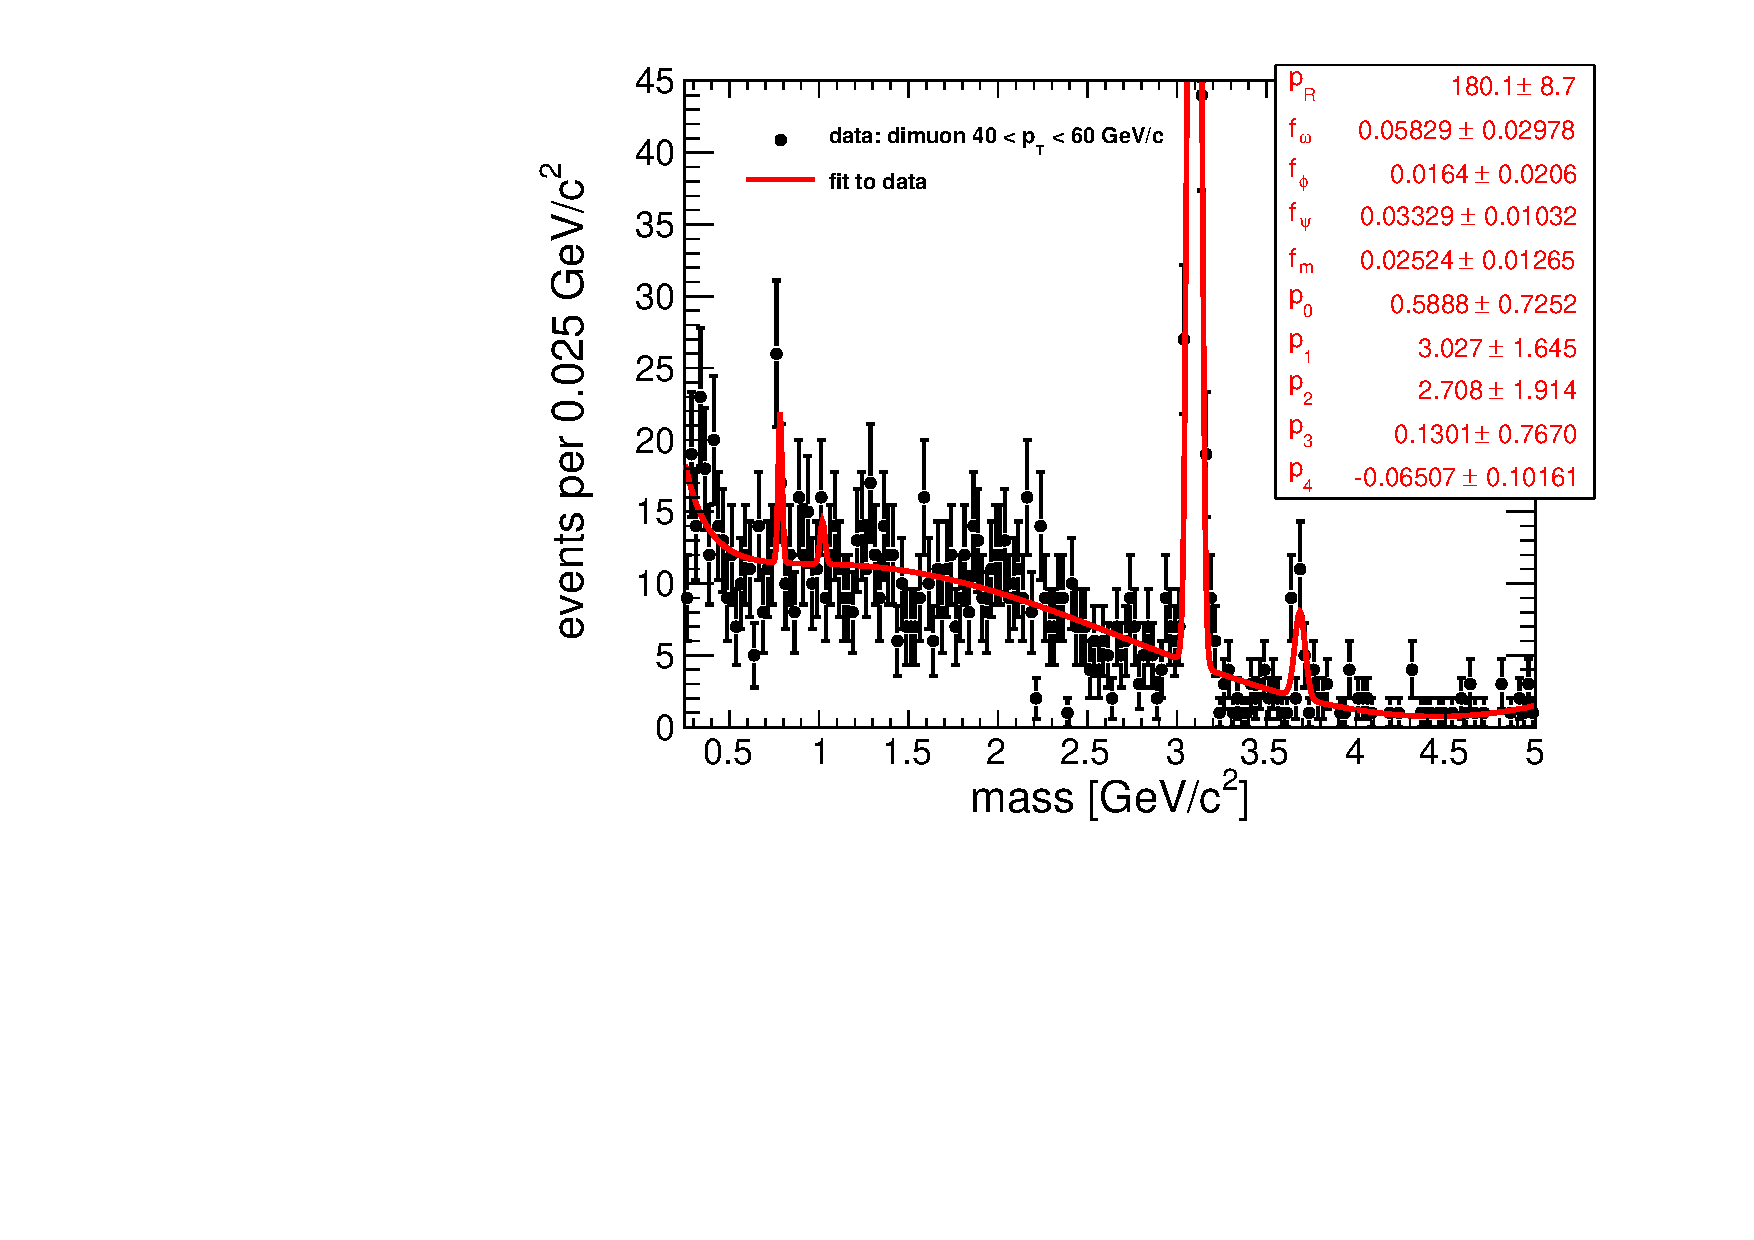
\includegraphics[width=0.5\linewidth]{backgroundEnriched_highpt.pdf}
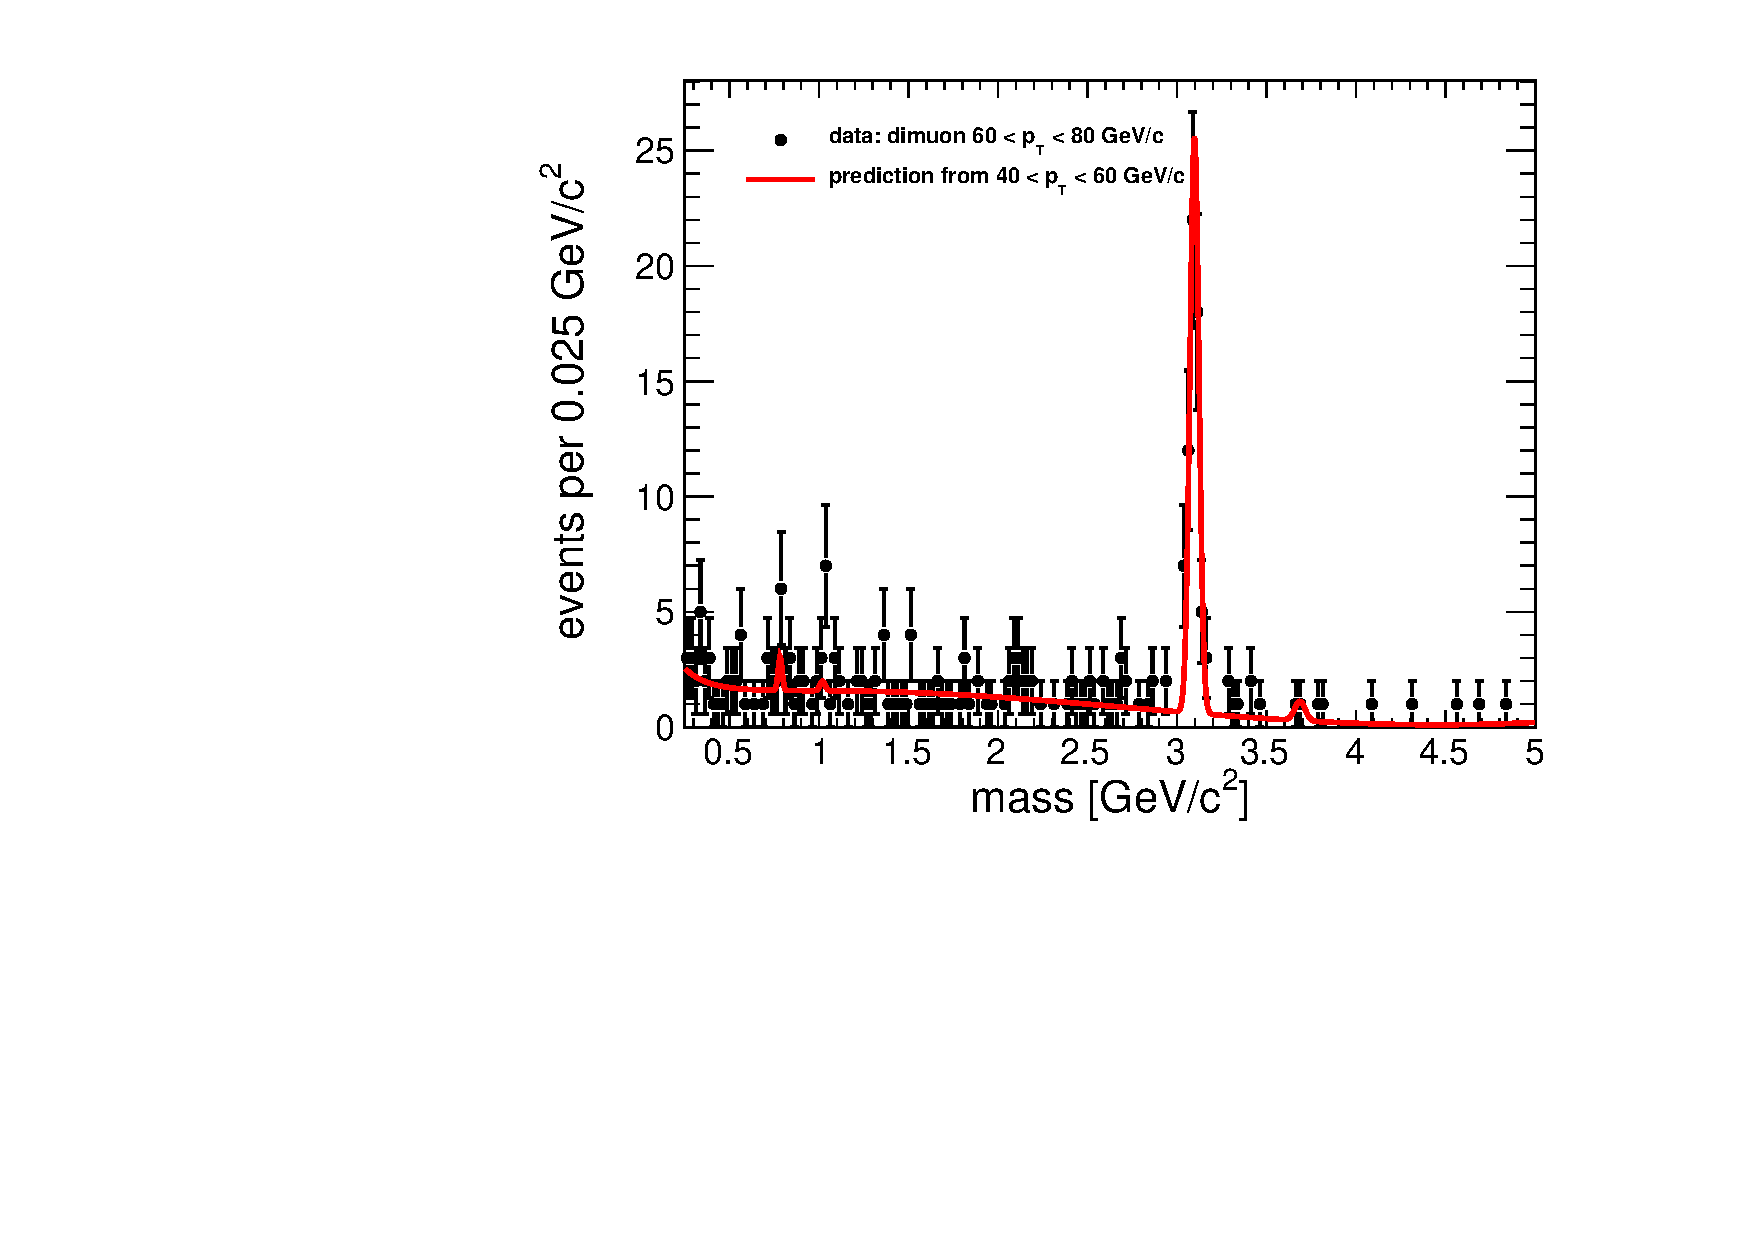
\includegraphics[width=0.5\linewidth]{control_highpt.pdf}
\end{frame}

\begin{frame}
\frametitle{Mass template for (a-2)}

\begin{itemize}
\item ``Background-enriched'' is 2 muons + 2 extra tracks, ``control''
  is 3 muons + 1 extra track.  (Extra tracks have the same kinematics
  as muons, but no associated muon segments.)

\item Of the 4 tracks, we plot the most consistent pair of dimuons.

\item Left: fit background-enriched to Eqn.~\ref{eqn:mass_template}
  with resonance fractions ($f_\omega$, $f_\phi$, $f_{\psi'}$) fixed
  to previous values and $p_{-1}$ released.

\item \textcolor{blue}{Blue MC:} dimuons with decay-in-flight or missing genlevel-match.

\item Right: control.  Ratio of normalization: $T_{3+1}(m) = 0.014 \, T_{2+2}(m)$.
\end{itemize}

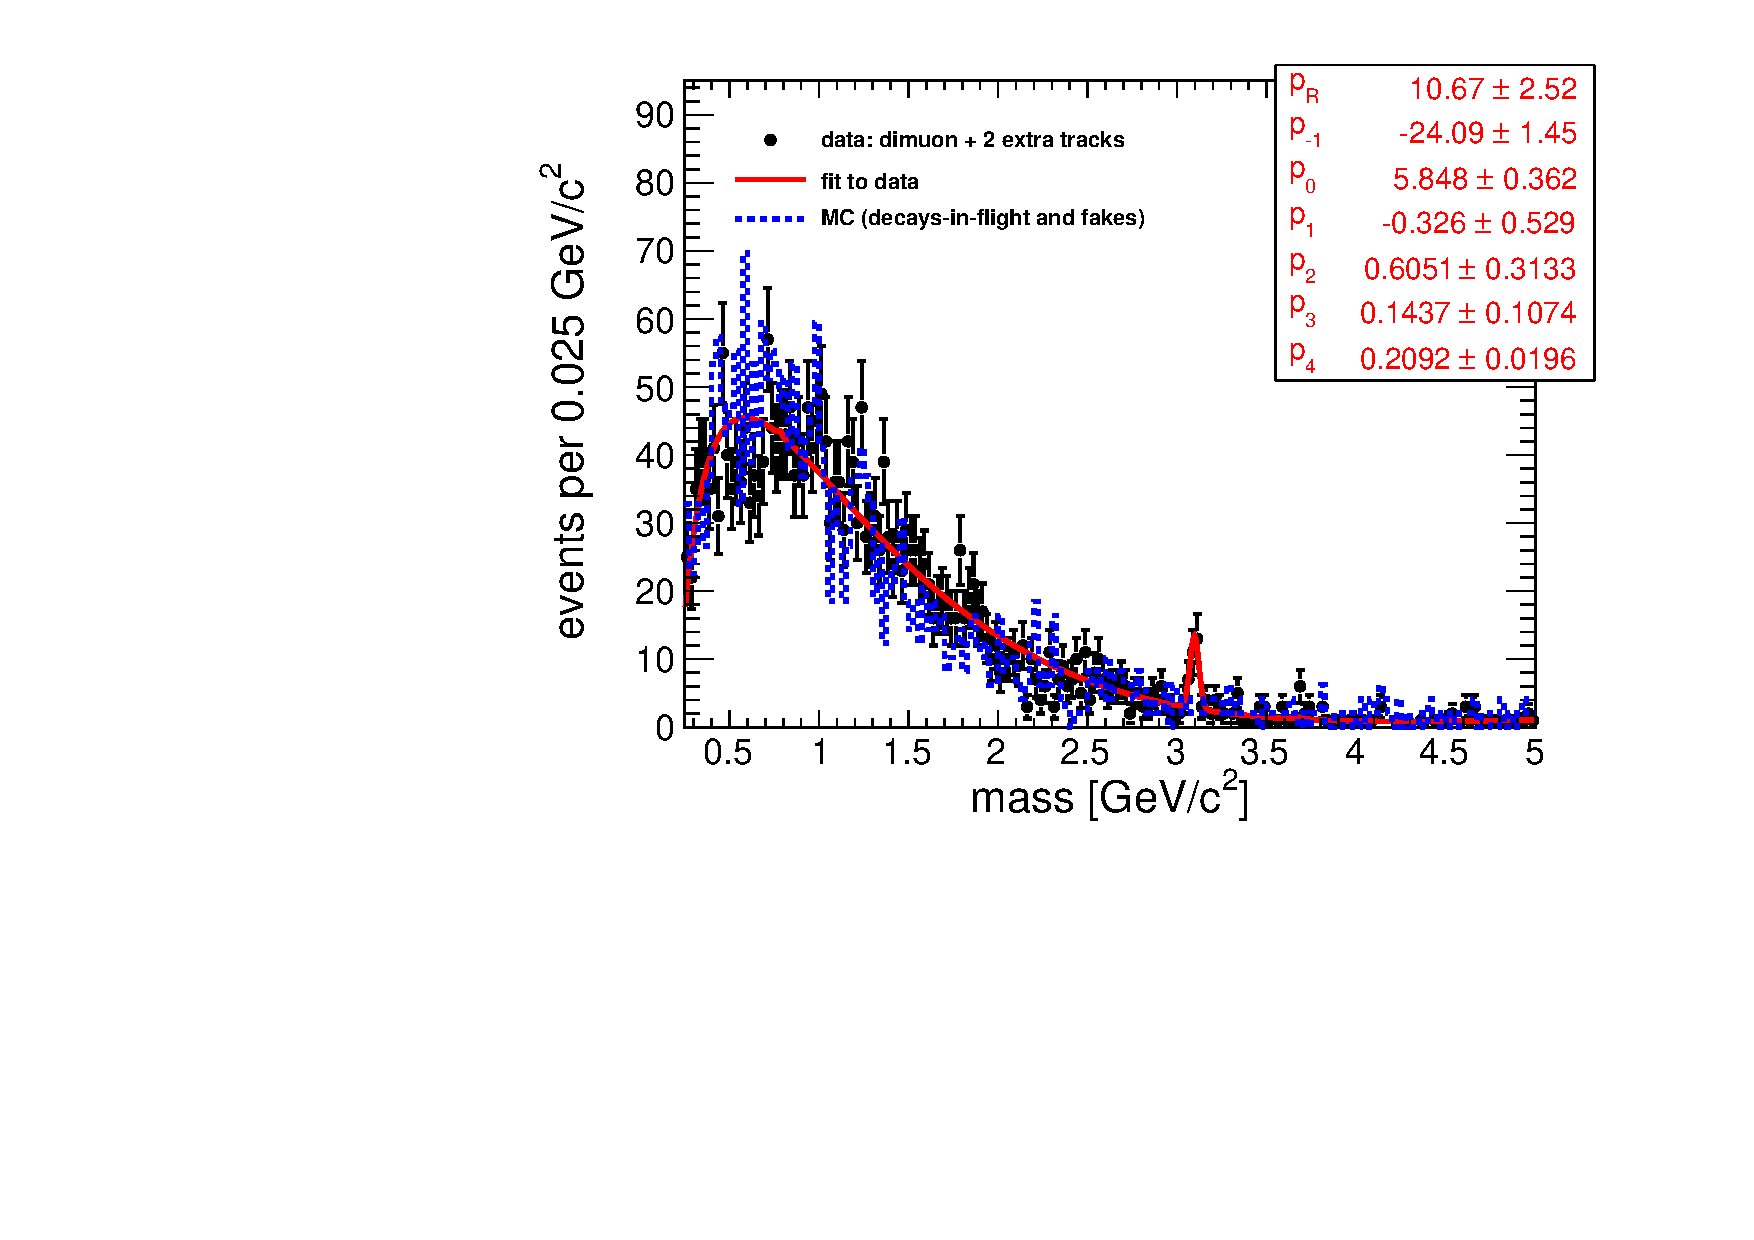
\includegraphics[width=0.5\linewidth]{backgroundEnriched_fakes.pdf}
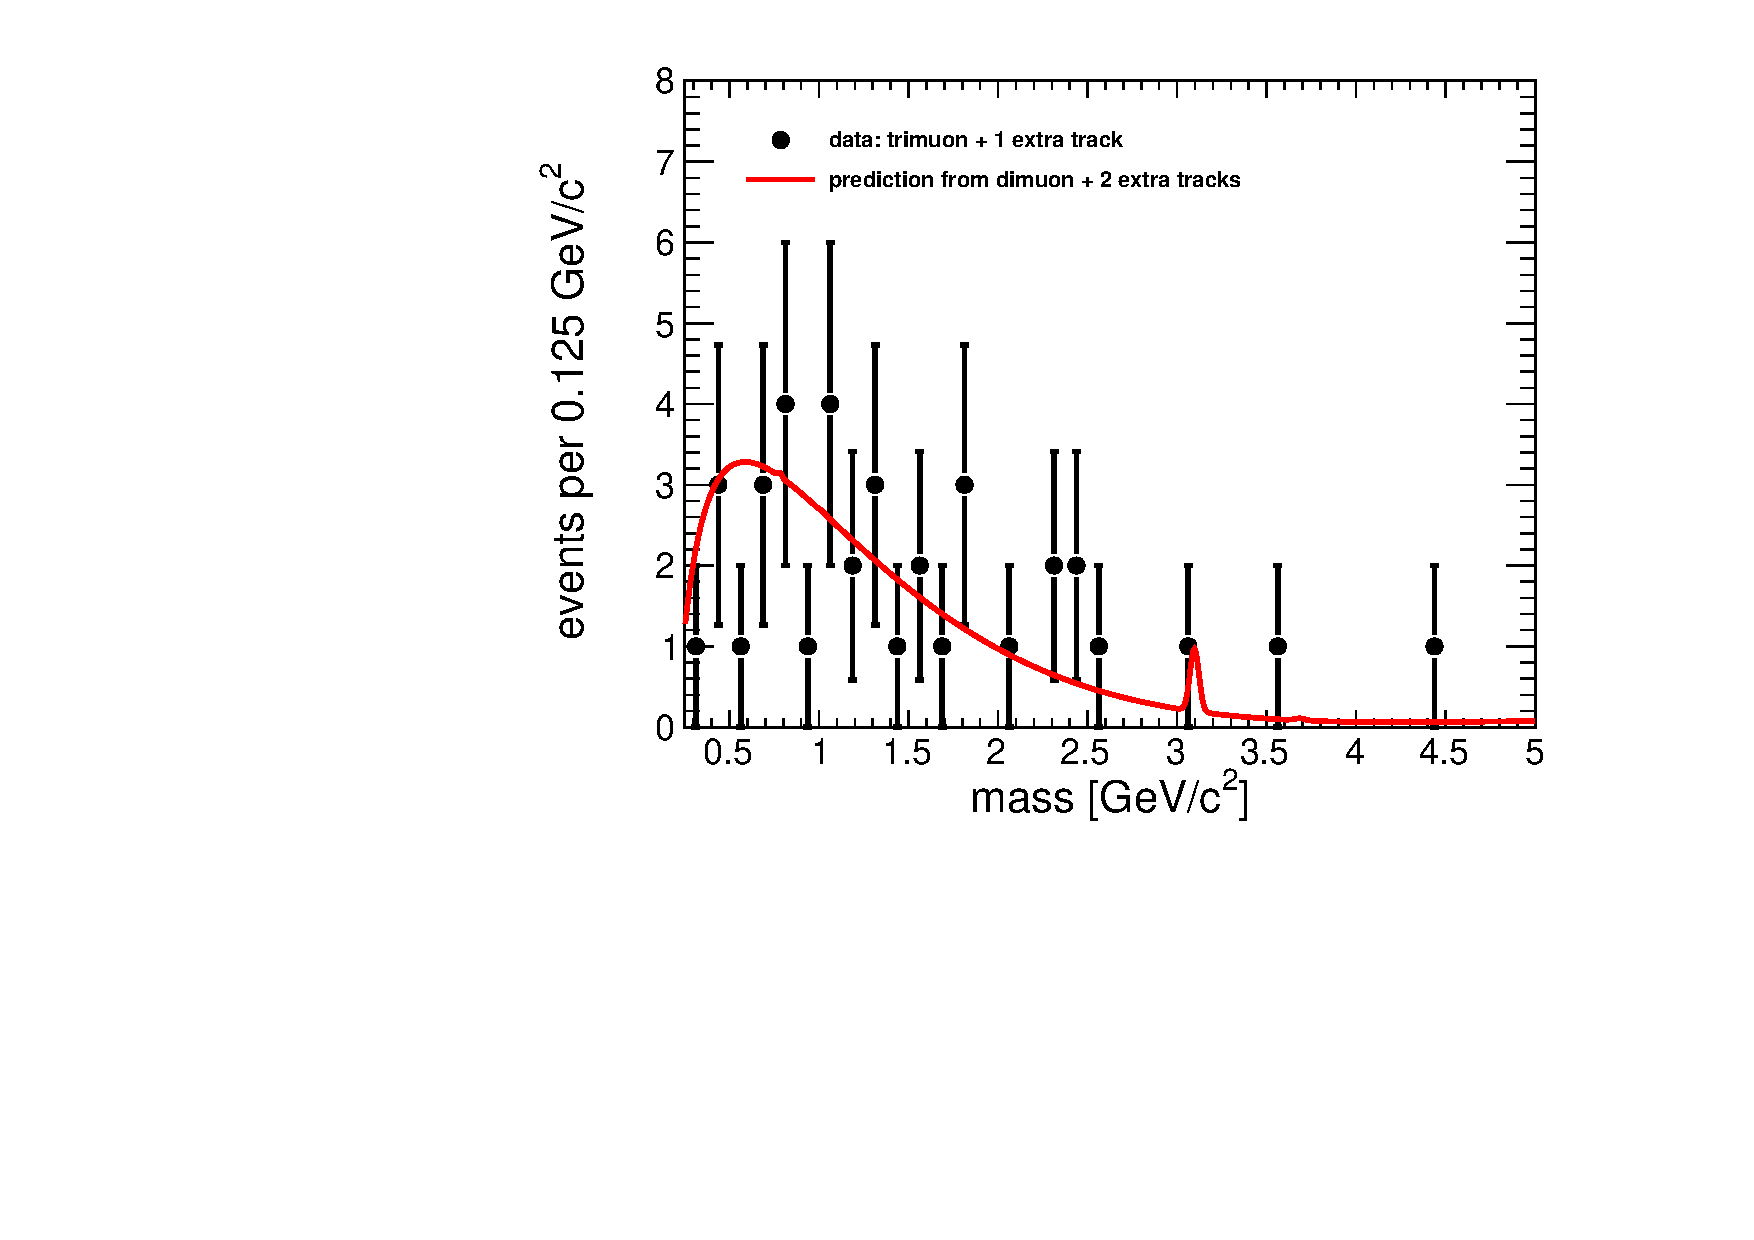
\includegraphics[width=0.5\linewidth]{control_fakes.pdf}
\end{frame}

\begin{frame}
\frametitle{Mass templates for (b-1)}

\begin{itemize}
\item ``Triggered dimuon'' contains the $p_T > 15$~GeV/$c$, $|\eta| <
  0.9$ muon, ``other dimuon'' is the other one.

\item ``Background-enriched'' sample for the triggered dimuon is the
  single-dimuon sample with $b\bar{b}$ cuts, ``background-enriched''
  for the other dimuon is dimuon + third muon satisfying the trigger.

\item Left: fit single-dimuon with $b\bar{b}$ cuts to
  Eqn.~\ref{eqn:mass_template} (only $p_{-1}$ fixed).  Right: fit
  dimuons + third muon sample with $f_\omega$, $f_\phi$, $f_{\psi'}$,
  $p_{-1}$ fixed.

\item \textcolor{blue}{Blue MC:} $b\bar{b}$ in the {\it signal}
  regions--- i.e., the difference between data-driven shapes and
  MC-driven shapes.
\end{itemize}

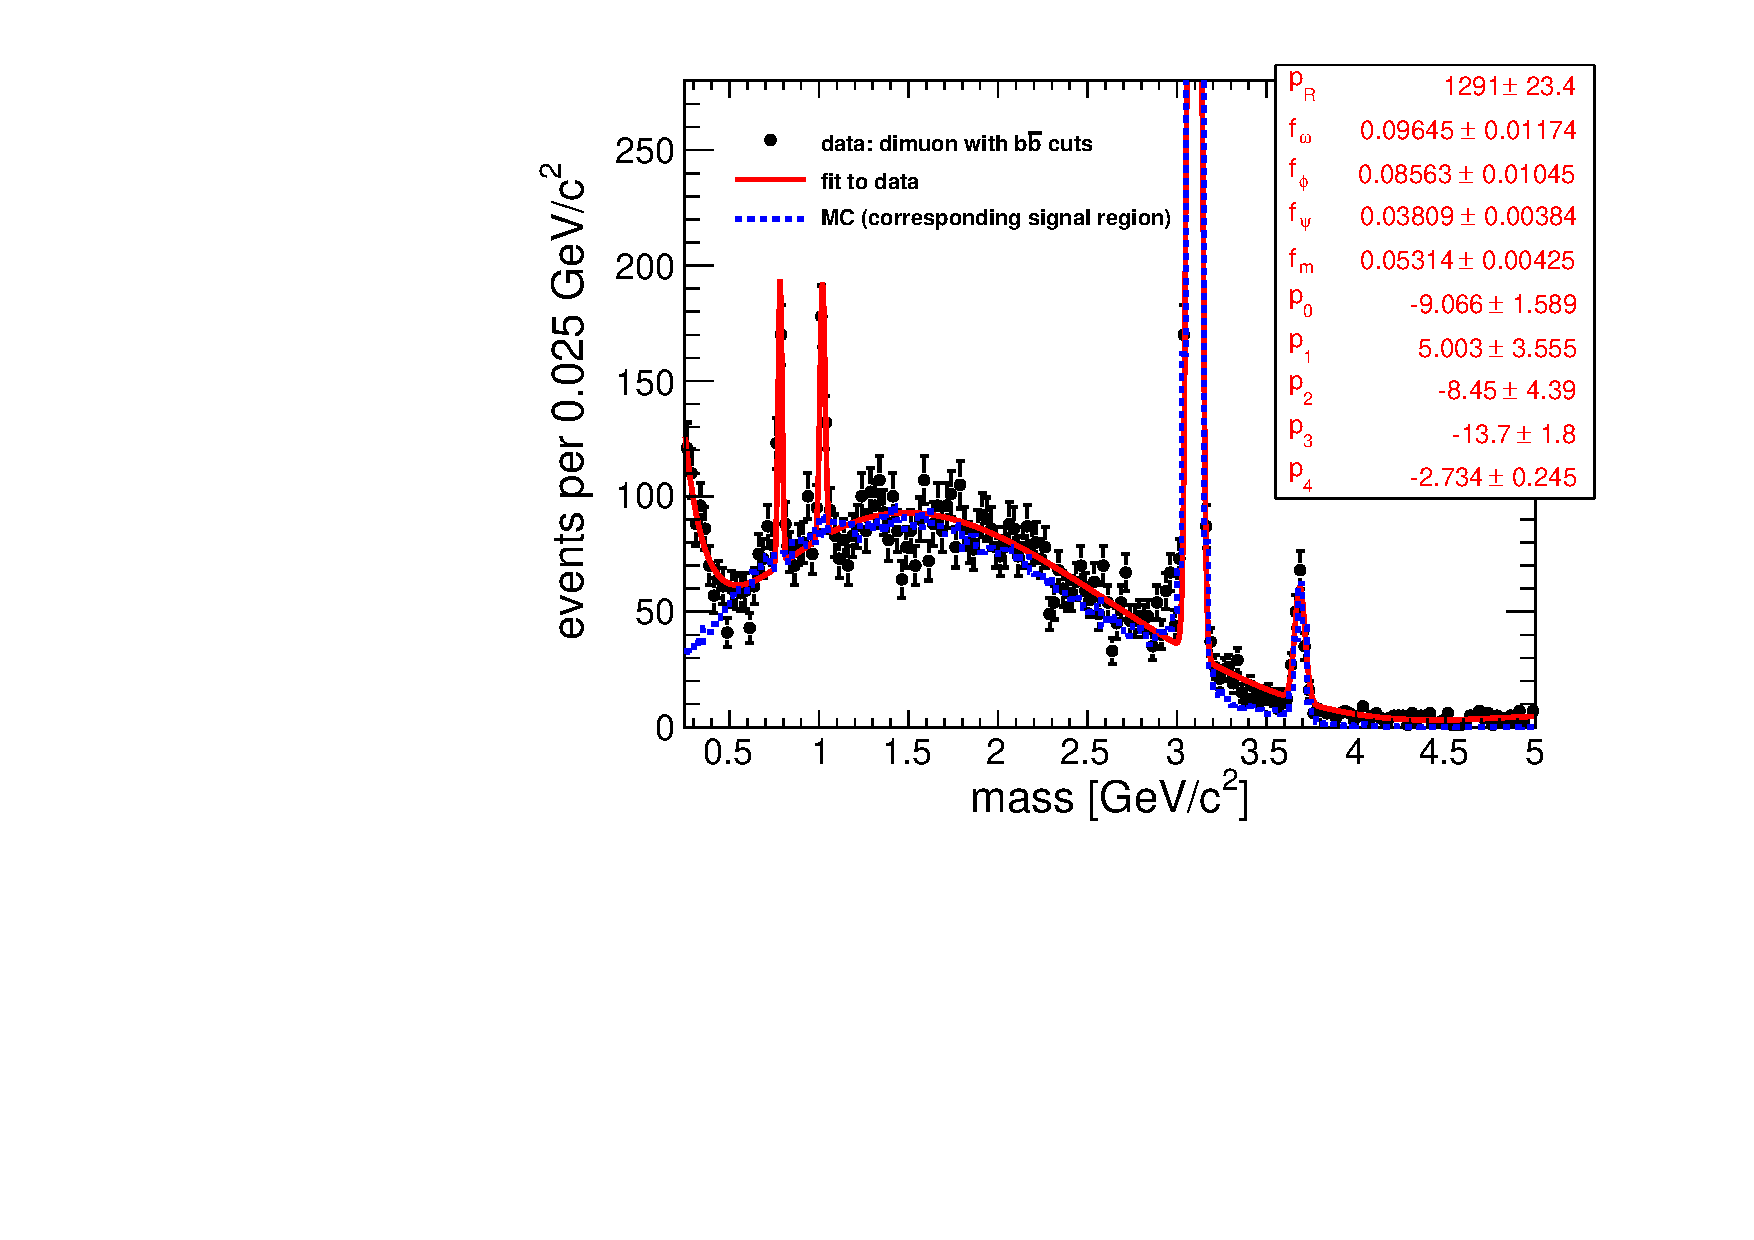
\includegraphics[width=0.5\linewidth]{backgroundEnriched_massC.pdf}
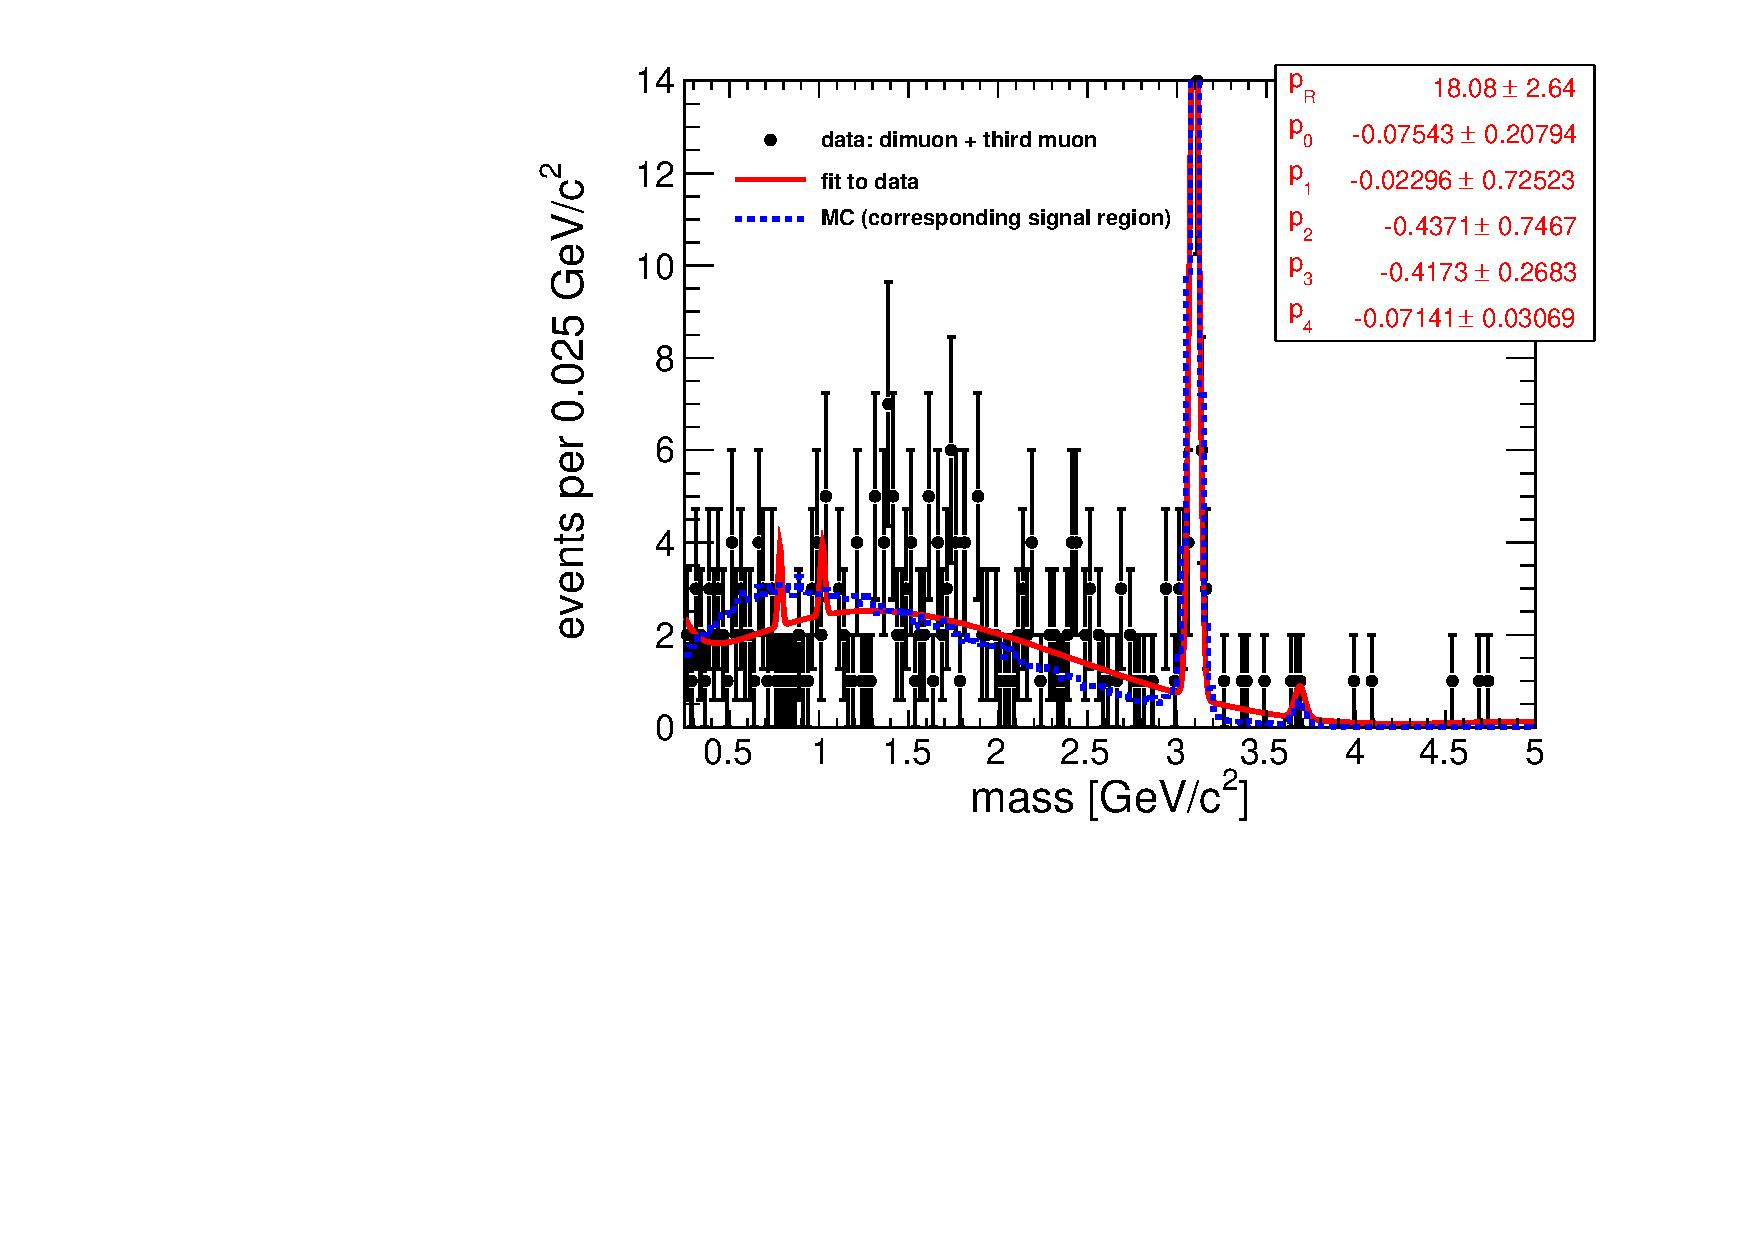
\includegraphics[width=0.5\linewidth]{backgroundEnriched_massF.pdf}
\end{frame}

\begin{frame}
\frametitle{Mass templates for (b-1)}

\begin{columns}
\column{0.5\linewidth}

\begin{itemize}
\item Control regions for both dimuons: select $J/\psi$ in one
  coordinate, plot non-$J/\psi$ in the other coordinate (right:
  $b\bar{b} \to 4\mu$ MC showing controls)
\item Bottom: projection of control MC and all MC, demonstrating that
  the 2-D \mbox{distribution factorizes\hspace{-1 cm}}
\end{itemize}

\column{0.5\linewidth}
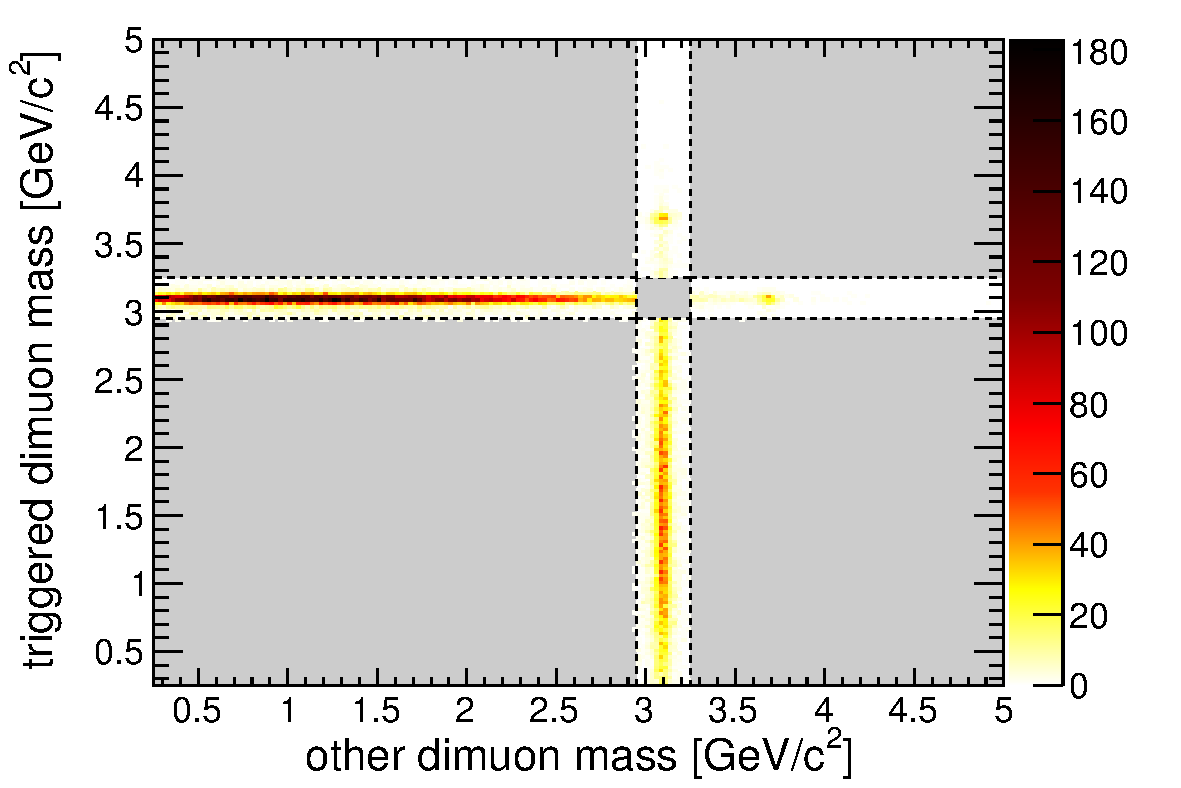
\includegraphics[width=\linewidth]{mc_controlregions.pdf}
\end{columns}

\vspace{0.25 cm}
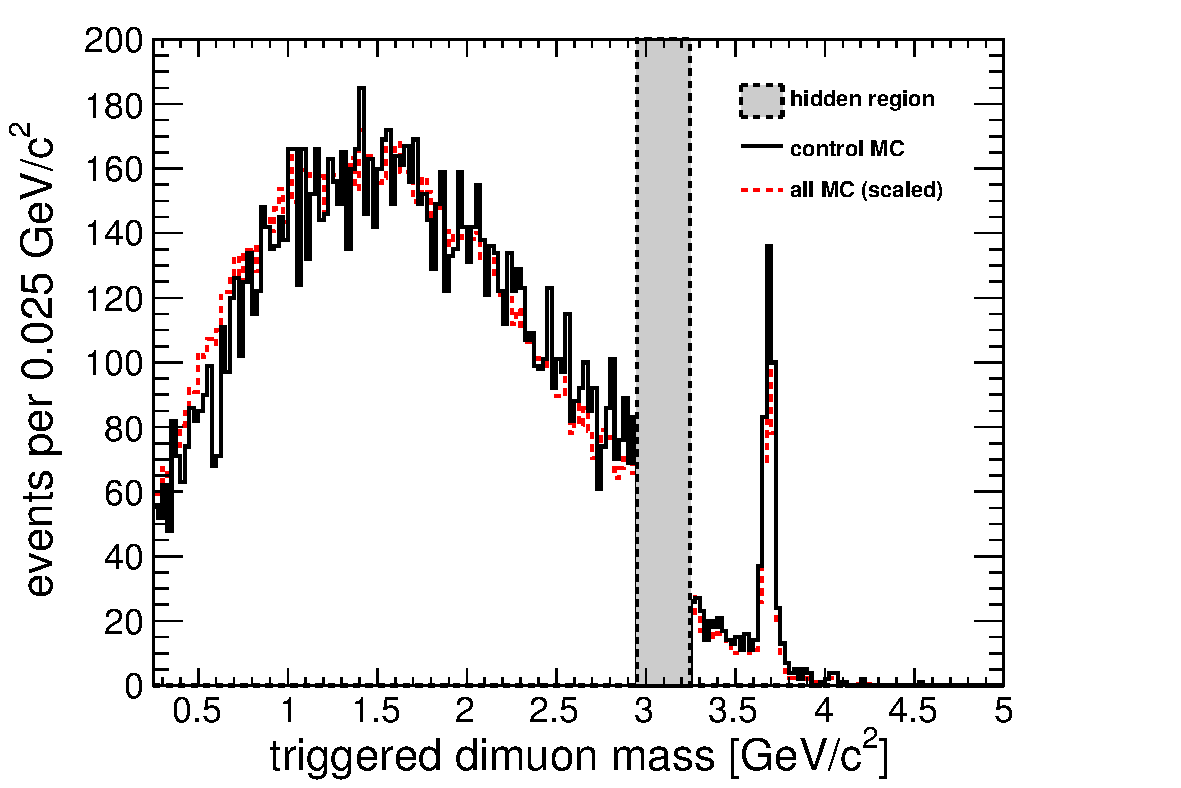
\includegraphics[width=0.5\linewidth]{mc_controlregions_factorize1.pdf}
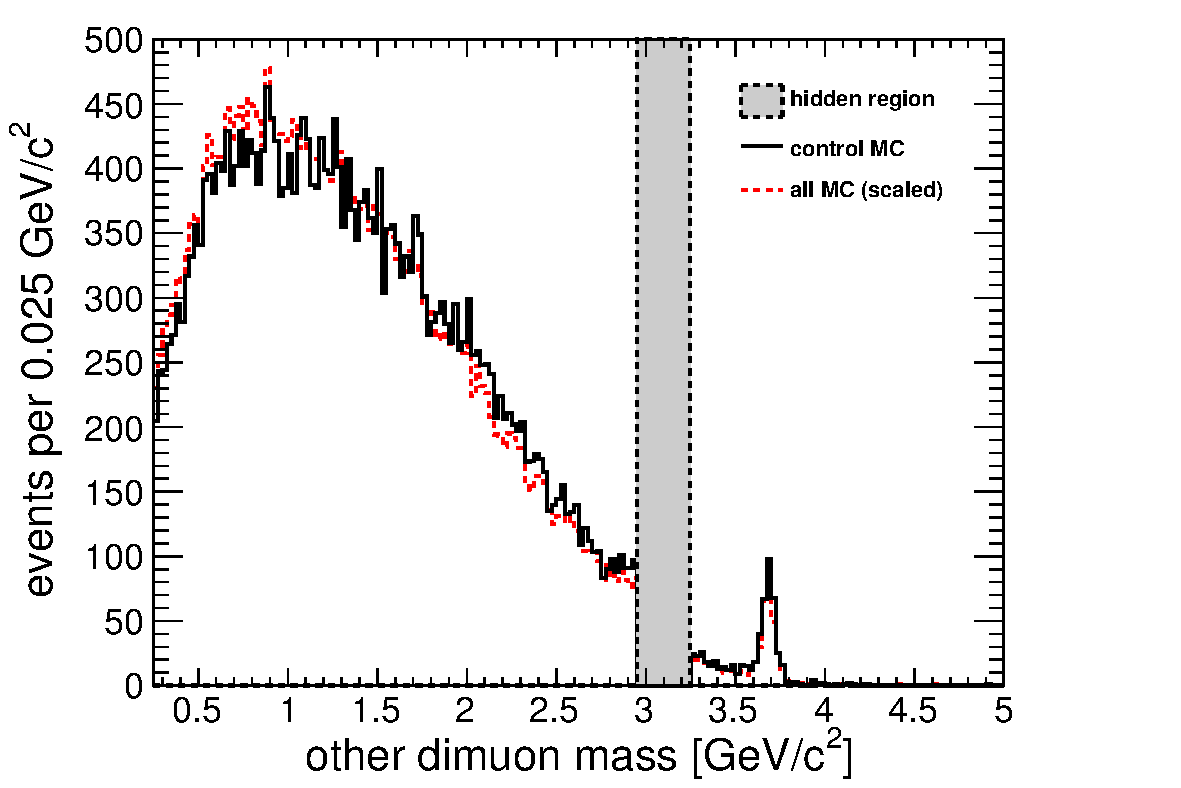
\includegraphics[width=0.5\linewidth]{mc_controlregions_factorize2.pdf}
\end{frame}

\begin{frame}
\frametitle{Mass templates for (b-1)}

\begin{itemize}
\item Control regions for data:
\end{itemize}

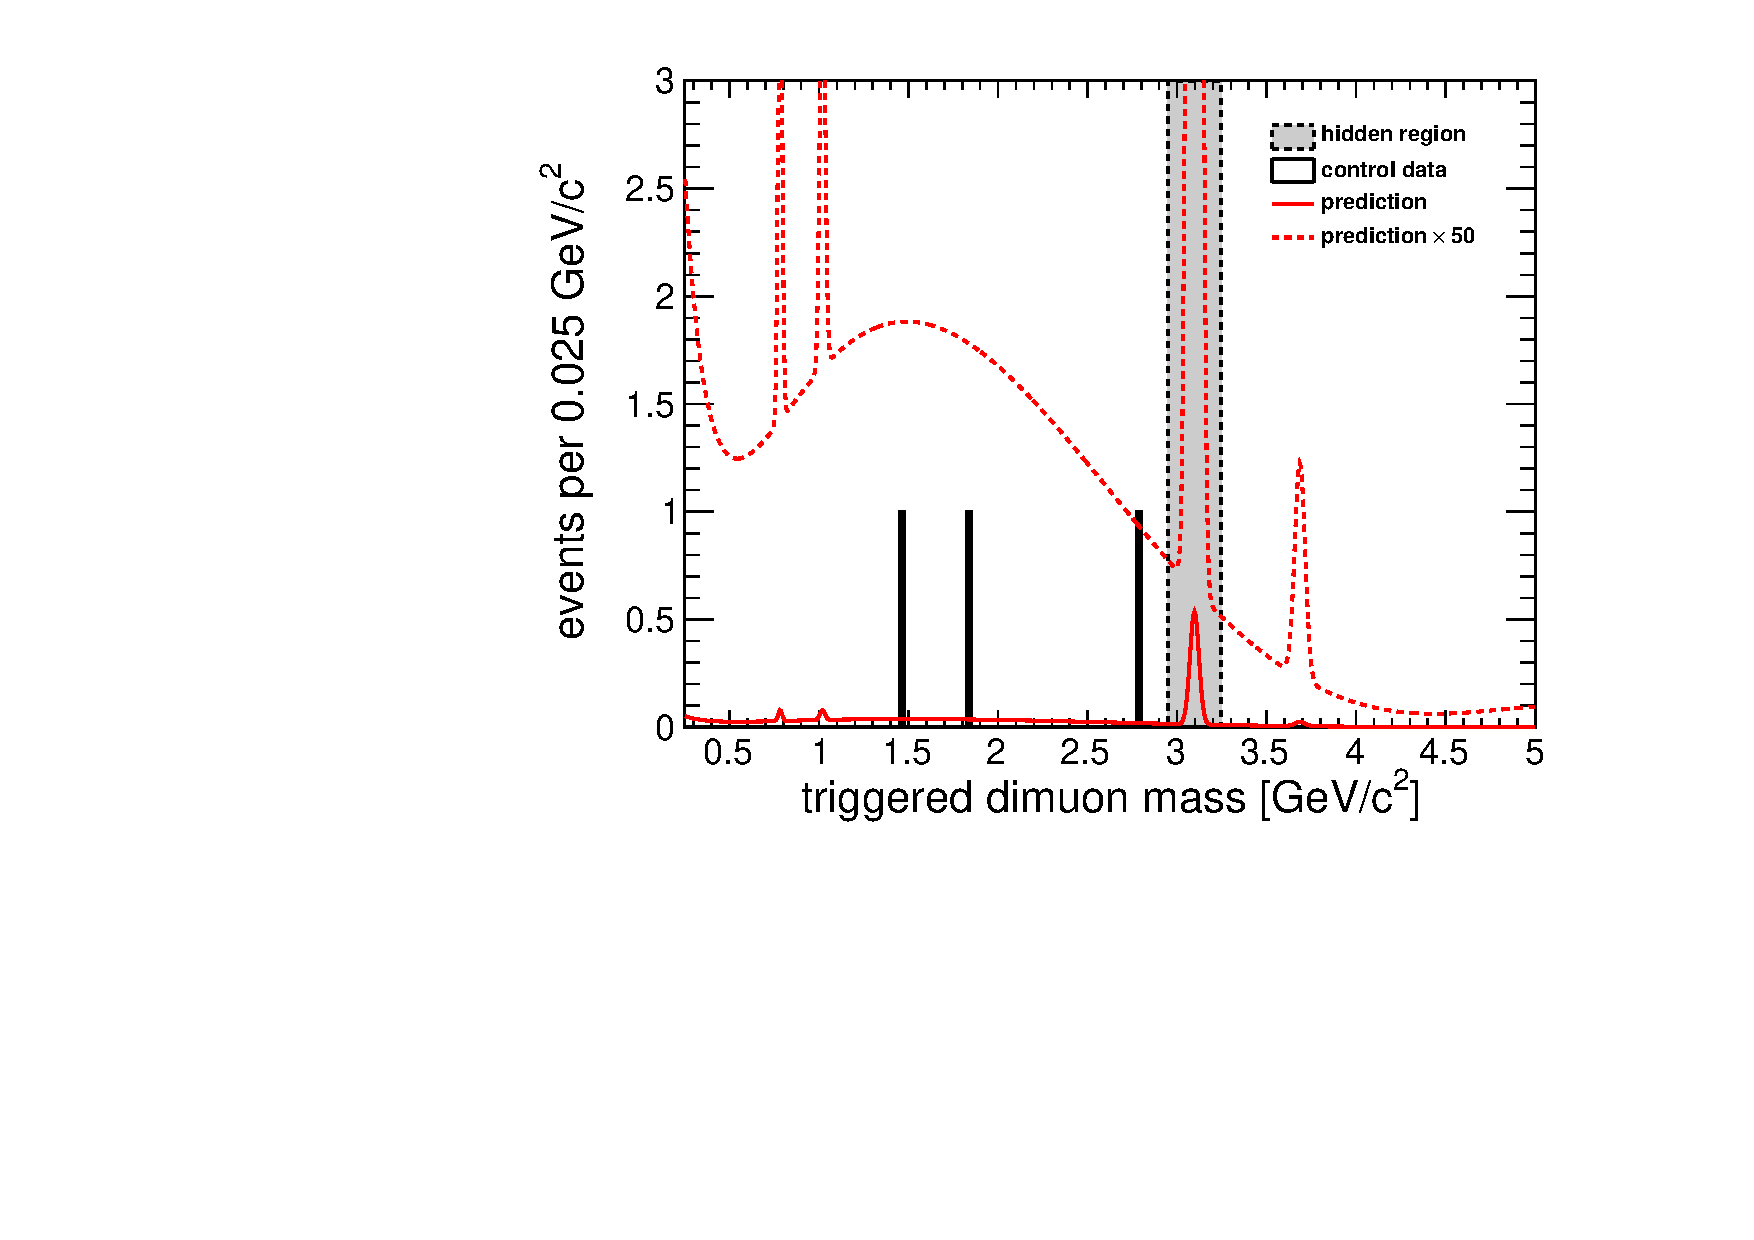
\includegraphics[width=0.5\linewidth]{control_massC.pdf}
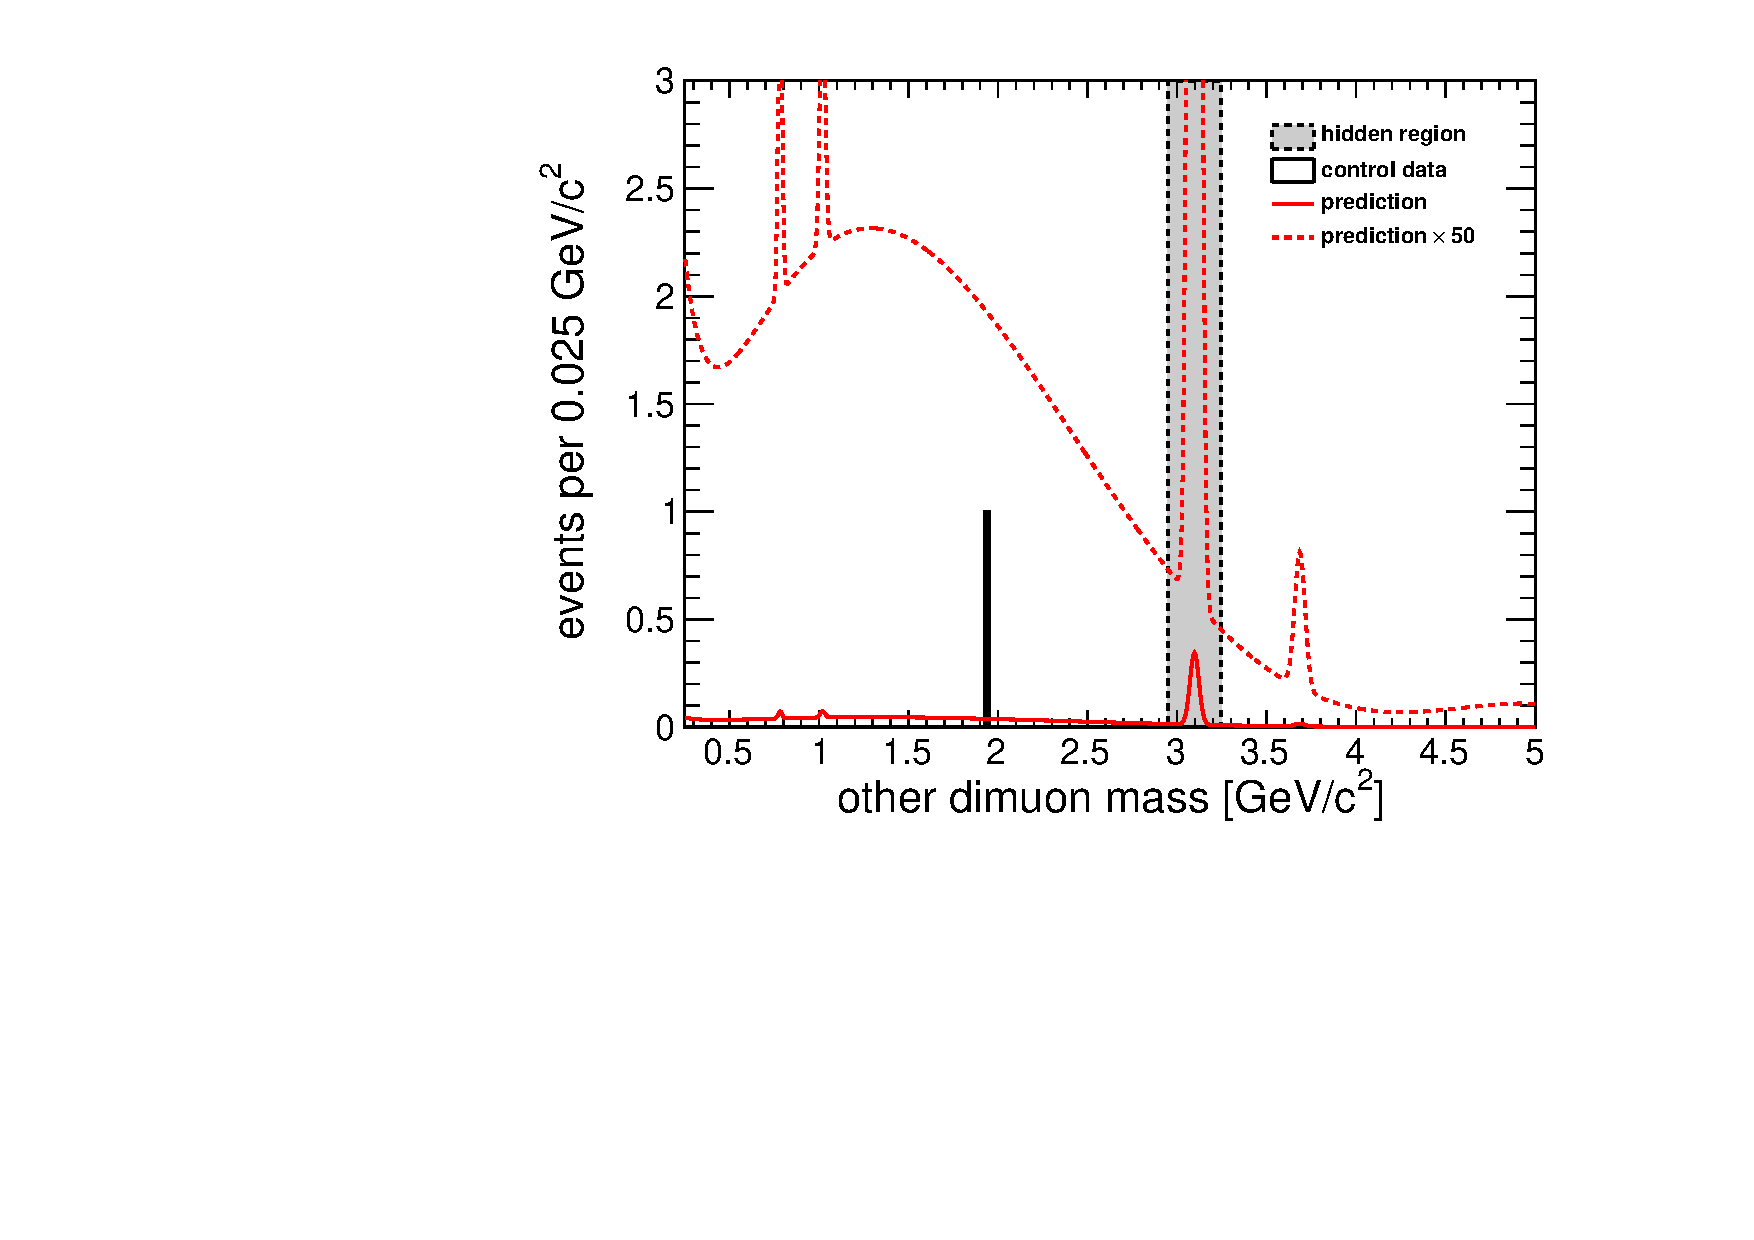
\includegraphics[width=0.5\linewidth]{control_massF.pdf}

\begin{itemize}
\item Normalization of $T_{td}(m)$, $T_{od}(m)$ for control regions:
\begin{itemize}
  \item $12\,841$ single $b \to 2\mu X$ events in background-enriched sample
  \item $\times$ 0.2\% probability for the other $b$ to go to $2\mu X$ (EvtGen)
  \item $\times$ 30\% in $J/\psi$ $\times$ 70\% not in $J/\psi$ (selected area in the plane)
\end{itemize}
= 5 events expected in each control region.  3 and 1 observed,
respectively.
\end{itemize}
\end{frame}

%% \begin{frame}
%% \frametitle{Outline}
%% \begin{itemize}\setlength{\itemsep}{0.75 cm}
%% \item 
%% \end{itemize}
%% %% \hspace{-0.83 cm} \textcolor{darkblue}{\Large Outline2}
%% \end{frame}

%% \section*{First section}
%% \begin{frame}
%% \begin{center}
%% \Huge \textcolor{blue}{First section}
%% \end{center}
%% \end{frame}

\begin{frame}
\frametitle{For the fitter:}
\begin{itemize}
\item Let the background normalization float!
\item Take the parameters from here; statistical errors for resonance fluctuations?
\item Late for the meeting\ldots
\end{itemize}
\label{numpages}
\end{frame}

\end{document}
